\chapter{Diseño del sistema de segmentación de cuerpos glaciares}
\doublespacing
%Esta sección se introduce el diseño y la implementación de un sistema que permita clasificar, segmentar y analisar el retroceso de cuerpos glaciares a partir de imagenes satelitales y comparar los resultados obtenidos de la estimación de retroceso de glacear QUelccaya con antecedentes previos. Involucra la selección de un algoritmo inteligente, base de datos, analisis de superficie de los cuerpos glaciares.
Esta sección presenta el diseño y la implementación de un sistema para la clasificación y segmentación de cuerpos glaciares a partir de imágenes satelitales. El sistema permite analizar el retroceso de la superficie glaciar y, finalmente, comparar los resultados de la estimación del retroceso del glaciar Quelccaya con estudios previos.


\begin{figure}[h!]
	\centering
	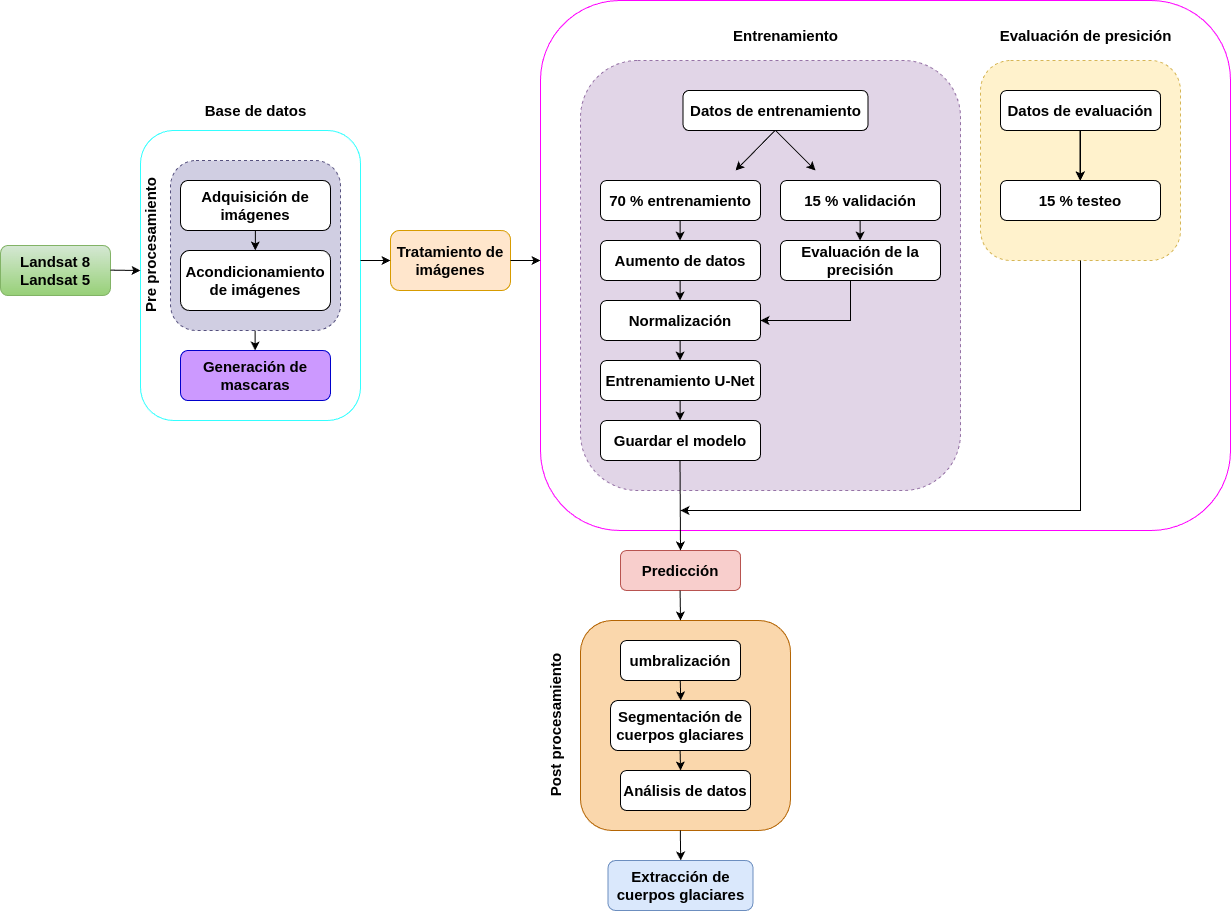
\includegraphics[width=0.95\linewidth]{graficos/flujo}
	\caption[Flujo de trabajo en este estudio.]{Flujo de trabajo en este estudio.
		
	}
	\label{fig:flujo}
\end{figure}

\begin{figure}[h!]
	\centering
	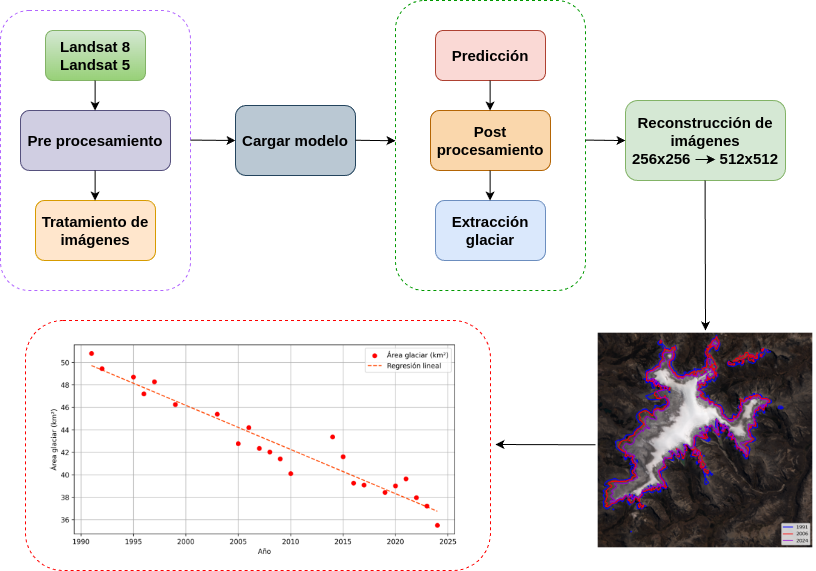
\includegraphics[width=0.9\linewidth]{graficos/flujo2}
	\caption[Procesamiento de datos para el analisis temporal.]{Procesamiento de datos para el analisis temporal.
		
	}
	\label{fig:flujo2}
\end{figure}


%\hl{Preguntas:
%¿En esta parte deberia considerarse el área de estudio?}

\section{Base de datos}
\begin{comment}
Para ralizar la implementación de un sistema inteligente a partir de deep learnig que permita clasificar y segmentar cuerpos glaciares, fue necesario contar con una adecuada base de datos, para ello se creó una base de datos a partir de imagenes del satelite Landsat 8 collection 2 Level-2 obtenidos a partir de U.S. Geological Survey (USGS) Earth Explorer \url{https://earthexplorer.usgs.gov/}. Landsat 8 esta equipada con el sensor Operational Land Imager (OLI)  mide en las porciones visibles, cercanas a infrarrojos y de onda corta del espectro. Sus imágenes tienen resoluciones espaciales multiespectramáticas y de 30 m a lo largo de una franja de 185 km de ancho, cubriendo amplias áreas del paisaje de la Tierra

\hl{Los productos de reflectancia de superficie Landsat 8 Operational Land Imager (OLI)se generan utilizando el algoritmo Land Surface Reflectance Code (LaSRC) (Versión 1.5.0).}

\hl{Reflectancia de la superficie

La reflectancia de la superficie (sin unidades) mide la fracción de la radiación solar entrante que se refleja desde la superficie de la Tierra hasta el sensor Landsat. Los algoritmos de reflectancia de la superficie LEDAPS y LaSRC corrigen los efectos de dispersión y absorción que varían temporal, espacial y espectralmente de los gases atmosféricos, los aerosoles y el vapor de agua, lo que es necesario para caracterizar de manera confiable la superficie terrestre.}


Según \parencite{perez2024exploratory} recomienda el uso datos de Landsat 8 Collection 2 Level-2, pues estos se somenten a la correción atmosferica para mediciones precisas de la reflactancia de la superficie.

La colección 2 ha mejorado la calidad de los datos en comparación con la colección 1, ya que tiene mejoras en la precisión de geolocalización absoluta, pero también incluye fuentes de modelado de elevación digital (DEM) actualizadas, calibración radiométrica mejorada y bandas de evaluación de calidad mejoradas, además de metadatos y formatos de archivo actualizados.

El nivel 2 son datos corregidos atmosféricamente (reflectancia de la superficie), mientras que el nivel 1 contiene un número digital (DN) escalado (generalmente enteros sin signo de 8 o 16 bits). El nivel 2 son los "datos listos para usar", ya que no es necesario implementar ninguna corrección.


 Cada pixel de la imagen multiespectral de landsa8 collection 2 level-2 es de 16 bits sin signo (UINT16). Este tipo de dato es usado para representar números enteros no negativos, ademas es eficienete en terminos de memoria, ya que cada píxel utiliza solo 16 bits (2 bytes de espacio). Un valor de 16 bits proporciona un rango amplio de valores, permitiendo almacenar una gran cantidad de información, lo cual es útil para capturar una variedad amplia de intencidad de luz reflejada o emitida. Ademas las implicaciones del tipo de datos UIN16 con respecto a la resolución radiométrica, permite una mayor precisión en la detección de diferencias sutiles en la reflectancia o emisión de la superficie terrestre. Esto es especialmente útil en estudios de cambios ambientales y monitoreo de la vegetación, cuerpos de agua, y suelos.
 
 \end{comment}
 
 Para implementar un sistema inteligente basado en deep learning que permita clasificar y segmentar cuerpos glaciares, es fundamental disponer de una base de datos adecuada. En este caso, se creó una base de datos utilizando imágenes del satélite Landsat 5 y Landsat 8 Collection 2 Level-1, obtenidas a través del Earth Explorer del U.S. Geological Survey (USGS) \url{https://earthexplorer.usgs.gov/}. 
 
 Según parte de la documentación oficial de USGS \parencite{usgs_landsat}, se recomienda el uso de datos de Collection 2 Level-1 para analisis temporal, debido a que estos datos se someten a correcciones atmosféricas, lo cual permite mediciones más precisas de la reflectancia. 
 
 Los productos de Landsat Level-1 consisten en números digitales (DN) calibrados y escalados que representan los datos de imágenes multiespectrales. Los datos de Nivel 1 se clasifican en una estructura basada en niveles. Los datos de Nivel 1 de nivel más alto se calibran radiométricamente y se corrigen geométricamente utilizando puntos de control terrestre (GCP) y datos de modelos de elevación digitales (DEM) para corregir el desplazamiento del relieve.

 
 %Además, cada píxel de las imágenes multiespectrales de Landsat 8 Collection 2 Level-2 es de 16 bits sin signo (UINT16). Este tipo de dato se utiliza para representar números enteros no negativos y es eficiente en términos de memoria, ya que cada píxel utiliza solo 16 bits (2 bytes de espacio). Un valor de 16 bits proporciona un amplio rango de valores, lo que permite almacenar una gran cantidad de información, útil para capturar una variedad extensa de intensidades de luz reflejada o emitida. Además, el uso de datos UINT16 tiene implicaciones en la resolución radiométrica, permitiendo una mayor precisión en la detección de diferencias sutiles en la reflectancia o emisión de la superficie terrestre. Esto es especialmente valioso en estudios de cambios ambientales y en el monitoreo de la vegetación, cuerpos de agua y suelos \parencite{usgs_landsat_2024}.
 
 %En este contexto, se descargaron imágenes multiespectrales de Landsat 8 Collection 2 Level-2 que contienen exclusivamente cuerpos glaciares.
 

%% https://gis.stackexchange.com/questions/439767/landsat-collections


\subsection{Adquisición de imágenes}
Para construir una base de datos a partir de imágenes satelitales Landsat, este estudio utiliza datos ópticos multiespectrales obtenidos de satélites. Se accedió a estos datos a través de la plataforma de acceso abierto del Servicio Geológico de los Estados Unidos (USGS). La política de datos abiertos y gratuitos de USGS Landsat se ha mantenido constante desde su implementación. Los datos de la Colección 2 de Landsat, en formato Level 1, están disponibles para su descarga a través de EarthExplorer. Solo es necesario visitar la página web de acceso a datos de Landsat para aprender cómo buscar y descargar todos los productos disponibles desde los portales de datos de USGS.


Se seleccionaron escenas 001/071, 002/070, 003/070, 004/069, 007/067, 008/066 capturadas por los sensores TM de landsat 5 desde el año 1990 hasta el año 2011, y del sensor OLI de Landsat 8 desde el año 2013 hasta el 2024. Cada escena tiene una resolución de 7721x7591 para Landsat 5 y una resolución de 7800 × 7600 píxeles para Landsat 8. Se consideraron los siguientes criterios de selección: todas las escenas debían haber sido adquiridas durante la estación seca, entre junio y septiembre, para minimizar posibles errores de clasificación debido a la presencia de nieve temporal. Además, las escenas debían tener un porcentaje de nubosidad inferior al 10 \%. Las escenas seleccionadas incluyen las Cordilleras Blanca, Huallanca, Huayhuash, Raura, Huagoruncho, La Viuda, Central, Huaytapallana, Chonta, Ampato, Urubamba, Vilcanota, Huanzo, Chila, La Raya, Vilcabamba, Carabaya, Apolobamba y la Cordillera Oriental en la Paz, Bolivia. 

%Para obtener información sobre la elevación del terreno, utilizamos el modelo de elevación digital (DEM) de Shuttle Radar Topography Mission (SRTM), con el proposito de calcular la distribución de área de elevación de las masas de hielo.


\begin{figure}[h!]
	\centering
	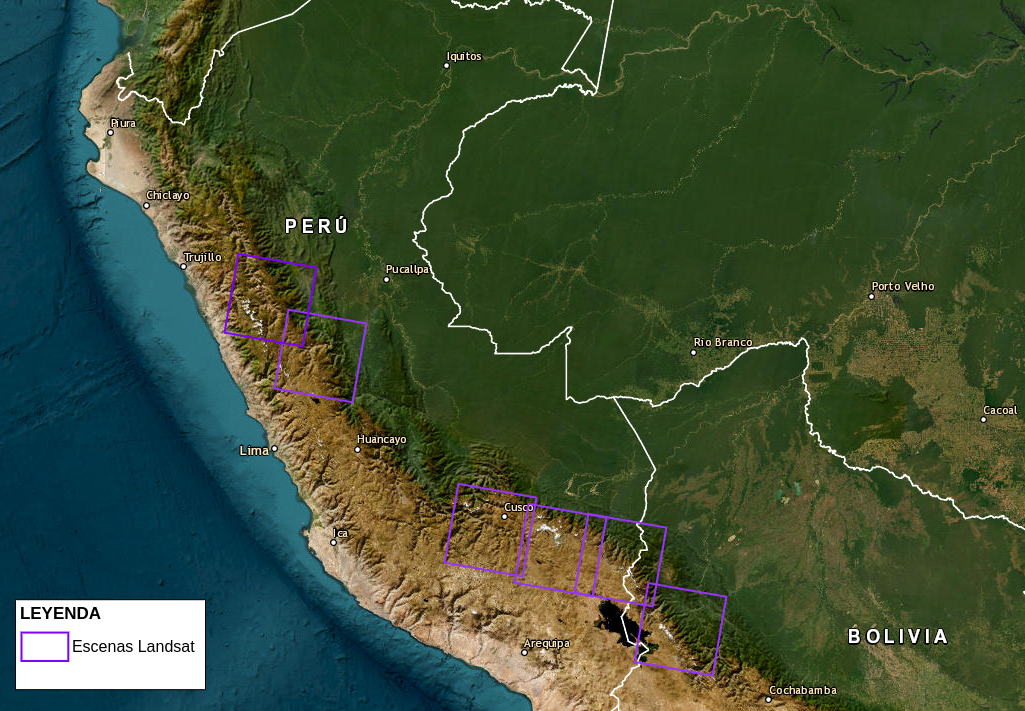
\includegraphics[width=\linewidth]{graficos/escena}
	\caption[Escenas de Landsat seleccionadas para el conjunto de datos.]{Escenas de Landsat seleccionadas para el conjunto de datos.
		
	}
	\label{fig:escena}
\end{figure}


\subsection{Acondicionamiento de las imágenes satelitales}
%\hl{Aqui necesitamos editar}

Al realizar la descarga de la escena seleccionada, se logran descargar las bandas 1, 2, 3, 4, 5 y 7 de Landsat 5 y las bandas 2,3,4,5,6,7 para Landsat 8, para ello se usa la metodología de \parencite{bezerra2023cloud}, \parencite{perez2024exploratory}. 

Primeramente es necesario convertir cada banda de DN a Reflactancia TOA, posterior a ello fue necesario apilar estas 6 bandas para tener una sola imagen multiespectral de 6 canales. 

%Para las imágenes muliespectrales de Landsat 6 se corrige la orientación de la imagen de 6 canales determinando su ángulo de inclinación mediante la transformada de Hough, la cual es útil para identificar conjuntos de puntos colineales en una imagen al mapear esos puntos a un conjunto de parámetros $(\theta, \rho)$ que definen una línea en el espacio de parámetros. El plano de búsqueda está limitado a un rango de  $[0, 180^\circ]$ para $\theta$  y desde $ [-R, R]$ para $\rho$. Esto permite delimitar un rectángulo que cubre la región de interés para la cuantificación. Con el ángulo de inclinación $\theta$ de la imagen satelital determinado, la imagen se rota de acuerdo con dicho ángulo. Posteriormente, se utiliza el algoritmo de detección de bordes de Canny para diferenciar los bordes de los datos de interés de aquellos que no son relevantes. Basándose en los bordes detectados, las áreas sin datos se eliminan y la imagen se divide en parches de 256 × 256 píxeles, lo que ayuda a reducir el costo computacional durante el entrenamiento. Este proceso se ilustra en la Figura.

Para corregir la orientación de las imágenes multiespectrales de Landsat 6 de seis canales, se determina el ángulo de inclinación de la imagen utilizando la transformada de Hough. Esta técnica es eficaz para identificar conjuntos de puntos colineales en una imagen, mapeando dichos puntos a un conjunto de parámetros $(\theta, \rho)$ que representan una línea en el espacio de parámetros. La búsqueda se restringe a un rango de $[0, 180^\circ]$ para $\theta$ y de $[-R, R]$ para $\rho$, lo cual permite definir un rectángulo que abarca la región de interés para cuantificar. Con el ángulo de inclinación $\theta$ establecido, se rota la imagen de satélite según este valor. Luego, el algoritmo de detección de bordes de Canny se aplica para distinguir los bordes relevantes de los irrelevantes. Con base en estos bordes detectados, se eliminan las áreas sin datos y se divide la imagen en parches de 256 × 256 píxeles, lo que reduce el costo computacional durante el entrenamiento. Este proceso se muestra en la Figura \ref{fig:RotationL8}.

Para las imágenes de Landsat 5 no es posible corregir la orientación utilizando la metodología anterior, debido a que los bordes de estas imágenes no son uniformes. Por este motivo, las imágenes se dividieron en parches de 256x256 píxeles manteniendo la misma posición de la imagen.

Finalmente las imágenes multiespectrales tienen una forma de 6x256x256 (numero de canales=6, ancho = 256, alto = 256), un tamaño adecuado para incluirlo en la base de datos. 

\begin{figure}[h!]
	\centering
	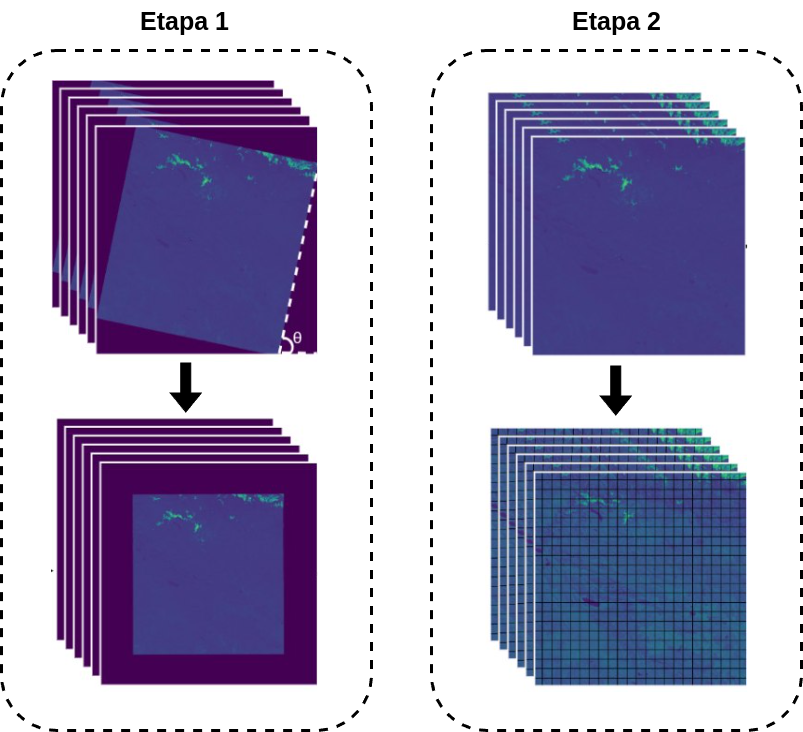
\includegraphics[width=0.7\linewidth]{graficos/acondicionamiento}
	\caption[Acondicionamiento de imágenes Landsat 8.]{Acondicionamiento de imágenes Landsat 8.
		
	}
	\label{fig:RotationL8}
\end{figure}
 
\subsection{Generación de máscaras}


%%Para crear las máscaras a partir de las imagenes multiespectrales de 6 canales, se considero el NDSI para segmentar cuerpos glaciares, sin embargo hubó lagos mal clasificados como áreas de cobertura glaciar, para ello se utilizo el NDWI que permitió segmentar cuerpos de agua, posteriormente se realizo una diferencia entre el NDSI y el NDWI, debido a que algunos cuerpos de agua son clasificados incorrectamente como áreas glaciares al realizar la diferencia entre NDSI y NDWI se eliminaron algunos pixeles que cubrian las zonas glaciares, para ello se tuvó que corregir las imagenes segmentadas de forma manual. Ademas se utilizo google aerth para verficar que la segmentación y la correcciones sean las más fidedignas posibles. Dicho proceso se observa en la figura. 
Las máscaras de cada imagen multiespectral solamente tienen que incluir cuerpos glaciares, para ello se utilizó el Índice de Diferencia de Nieve Normalizado (NDSI, por sus siglas en inglés) con el objetivo de segmentar los cuerpos glaciares. Sin embargo, durante este proceso, algunos lagos fueron erróneamente clasificados como áreas de cobertura glaciar debido a sus características espectrales similares a la nieve y el hielo como se muestra en la Figura \ref{fig:agua_sombra}b. Para corregir este problema, se empleó el Índice de Diferencia de Agua Normalizado (NDWI, por sus siglas en inglés), el cual es más adecuado para la identificación de cuerpos de agua.

Posteriormente, se calculó la diferencia entre los valores del NDSI y el NDWI para mejorar la precisión de la segmentación. Este enfoque ayudó a reducir la confusión espectral entre los lagos y las zonas glaciares, atenuando la clasificación incorrecta de algunos píxeles que, debido a su similitud espectral, habían sido clasificados erróneamente como glaciares en el resultado original del NDSI. Para eliminar completamente estos píxeles mal clasificados, se estableció un umbral de 0.67, que permitió diferenciar los píxeles correspondientes a cuerpos de agua de aquellos clasificados como glaciares.

No obstante, este método también provocó la eliminación de algunos píxeles que, en realidad, pertenecían a áreas glaciares. Por lo tanto, fue necesario realizar una corrección manual en las imágenes segmentadas para garantizar la precisión de la clasificación final. Para ello se binarizó la imagen segmentada, posteriormente se corrigieron las imágenes binarias empleando Google Earth para verificar la segmentación y las correcciones aplicadas, asegurando que el resultado final fuera lo más fiel posible a la realidad. Este proceso se ilustra en la Figura \ref{fig:Mask_Creating}, donde se puede observar la mejora en la identificación de las áreas glaciares y de los cuerpos de agua tras la aplicación de ambos índices y las correcciones manuales correspondientes.

Finalmente se obtuvieron máscaras que tienen una forma de 1x256x256 (numero de canales=1, ancho = 256, alto = 256), para Landsat 8 y Landsat 5, un tamaño adecuado para incluirlo en la base de datos.
\begin{comment}
	\begin{figure}[h!]
		\centering
		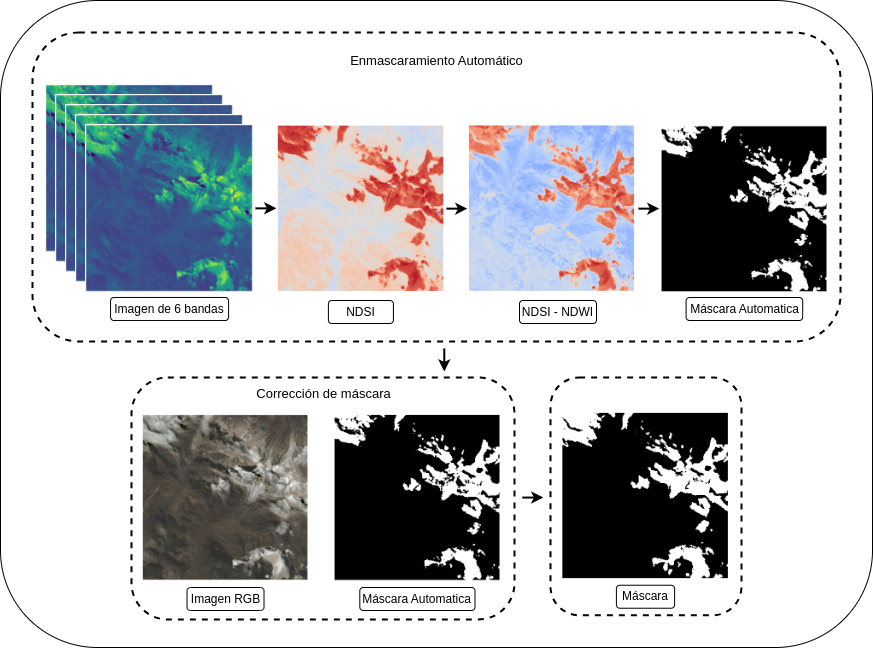
\includegraphics[width=\linewidth]{graficos/Mask_Creating}
		\caption[Proceso de creación de máscaras]{Proceso de creación de máscaras.
			
		}
		\label{fig:Mask_Creating}
	\end{figure}contenidos...
\end{comment}
\begin{figure}[h!]
	\centering
	\includegraphics[width=0.9\linewidth]{graficos/agua_sombra}
	\caption[Corrección de agua y sombras.]{Corrección de agua y sombras. a) Imagen RGB. b) Índice NDSI, se observa que los cuerpos de agua también son segmentados. c) NDSI-NDWI. d) Visualización de sombras. El área circular rojo encierra lagos, el verde encierra sombras y el morado encierra píxeles que aún tienen alto valor y necesitan ser eliminados.}
	\label{fig:agua_sombra}
\end{figure}
\begin{figure}[h!]
	\centering
	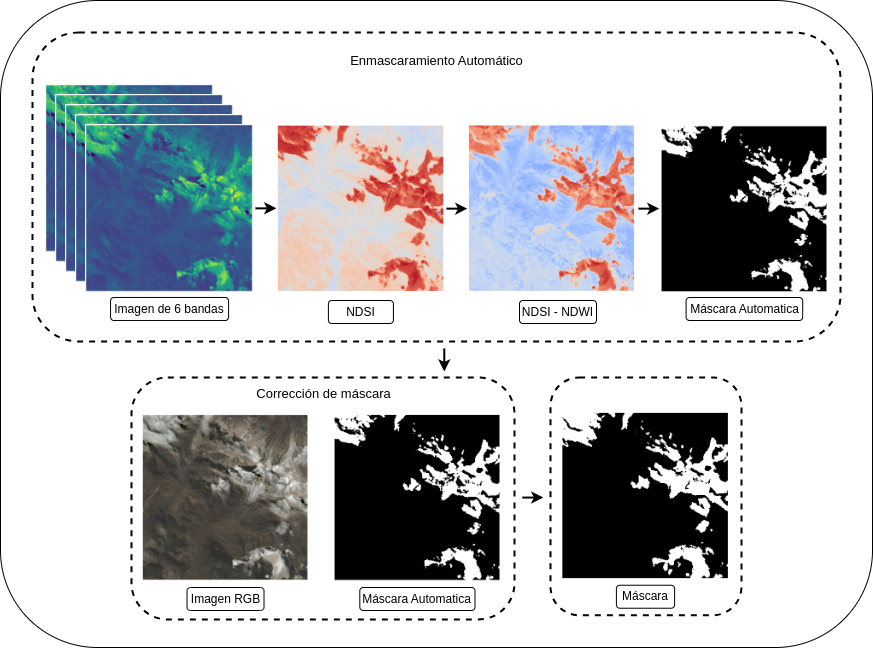
\includegraphics[width=\linewidth]{graficos/Mask_Creating}
	\caption[Proceso de creación de máscaras]{Proceso de creación de máscaras.}
	\label{fig:Mask_Creating}
\end{figure}
%\vspace{-10pt} % Ajusta según el espacio necesario

\subsection{Tratamiento de imágenes}

Las imágenes multiespectrales y sus respectivas máscaras para el conjunto de datos solamente deben incluir áreas glaceares, cada pixel de la imagen multiespectral para Landsat 8 es de 16 bits sin signo (UINT16) y 8 bits sin signo (UINT8) sin signo para Landsat 5, lo que implica que los valores de los píxeles en estas bandas pueden variar desde 0 hasta 65535 y 0 hasta 255 respectivamente. Cuando se procesan imágenes, especialmente para análisis avanzados como algoritmos de deep learning o procesamiento digital de señales, los datos se convierten a menudo a float64 o float32 para facilitar las operaciones matemáticas. Convertir los datos a un formato de punto flotante permite realizar calculos mas precisos y evitar errores de redondeo que pueden ocurrir con los datos de menor presición. 

Una práctica estándar en el procesamiento de imágenes y aprendisaje automático es normalizar los datos de imágenes a [0, 1] puesto que se mejora la eficiencia y efectividad del entrenamiento del modelo, garantiza la comparabilidad entre diferentes conjuntos de datos, evita problemas numéricos, y asegura que los modelos de machine learning y deep learning funcionen de manera óptima.

\section{Arquitecturas de aprendizaje profundo (Deep learning)}
%\subsubsection{1. Procesamiento del dataset}

%Las imágenes multiespectrales del conjunto de datos tienen una forma de 6x256x256 (numero de canales=6, ancho = 256, alto = 256) y las mascaras una forma de 1x256x256 (numero de canales=1, ancho = 256, alto = 256), para Landsat 8 y Landsat 5 cada pixel de la imagen multiespectral es de 16 bits sin signo (UINT16) y 8 bits sin signo (UINT8) sin signo respectivamente, lo que implica que los valores de los píxeles en estas bandas pueden variar desde 0 hasta 65535 y 0 hasta 255. Cuando se procesan imágenes, especialmente para análisis avanzados como algoritmos de aprendizaje profundo o procesamiento digital de señales, los datos se convierten a menudo a float64 o float32 para facilitar las operaciones matemáticas. Convertir los datos a un formato de punto flotante permite realizar calculos mas precisos y evitar errores de redondeo que pueden ocurrir con los datos de menor presición. 

%Una práctica estándar en el procesamiento de imágenes y aprendisaje automático es normalizar los datos de imágenes a [0, 1] puesto que se mejora la eficiencia y efectividad del entrenamiento del modelo, garantiza la comparabilidad entre diferentes conjuntos de datos, evita problemas numéricos, y asegura que los modelos de machine learning y deep learning funcionen de manera óptima.
%Para esté trabajo se utiliza el frameworks de Pytorch, para ello es necesario que nuestros datos sean convertidos a tensores de Pytorch.

\subsection{Implementación de la arquitectura de deep learning}

Se propuso 3 arquitecturas de segmentación semántica (U-Net, DeepResUNet y DeepLabV3Plus), para ello se implementó una red neuronal para cada modelo basandose en su arquitectura, dichas arquitecturas se muestran en las Figuras \ref{fig:unet2Arquitectura}, \ref{fig:RESUNET_Arquitectura} y \ref{fig:DeepLabv3plusArquitectura}. El tamaño de la imagen de entrada para cada arquitectura fue de 256x256 px.

El progreso de la segmentación semántica podría definirse como una tarea de clasificación a nivel de pixel para clasificar esos píxeles en cuerpos glaciares u otras clases. Las imágenes de los cuerpos glaciares segmentados con la máscara se compararon para minimizar la diferencia entre ellas durante el entrenamiento utilizando la pérdida de Dice. Se utilizaron Dice Coficcient, mean Intersegtion Union (mIoU) y Pixel Accuracy (PA) como métricas.

Donde [0,1] representa el valor de la probabilidad predicha alcanzada por el modelo para la clase de verdad fundamental con etiqueta = 1.

\begin{figure}[h!]
	\centering
	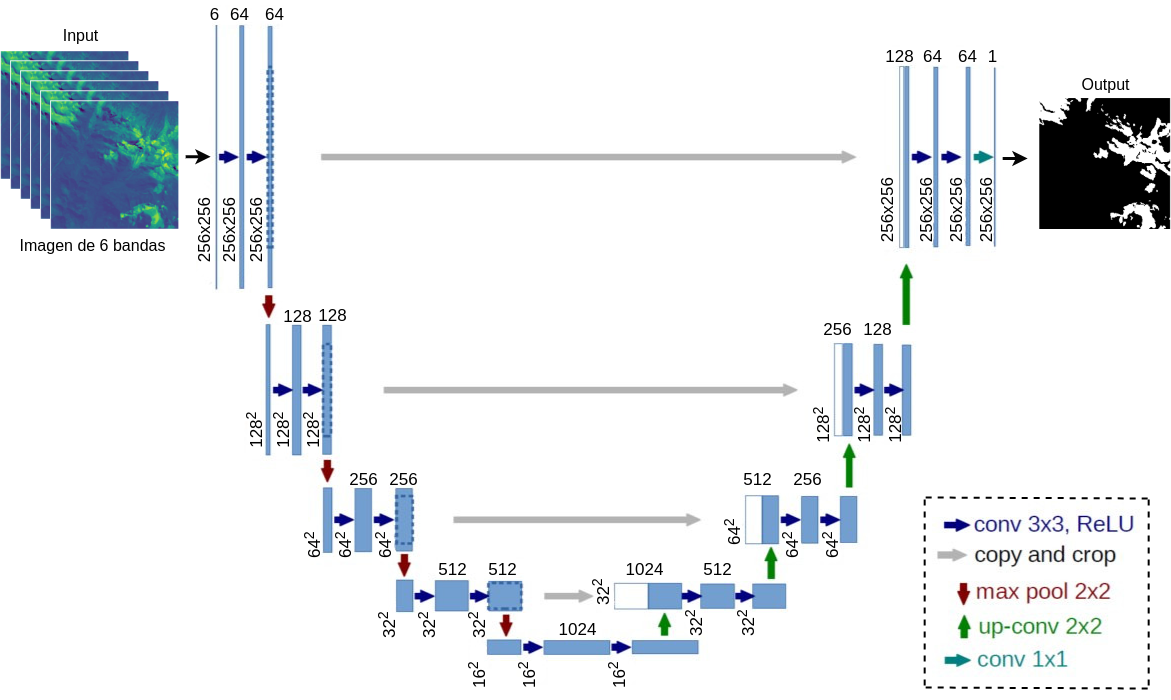
\includegraphics[width=0.7\linewidth]{graficos/unet2Arquitectura}
	\caption[Arquitectura del modelo U-Net]{Arquitectura del modelo U-Net.
		

	}
	\label{fig:unet2Arquitectura}
\end{figure}

\begin{figure}[h!]
	\centering
	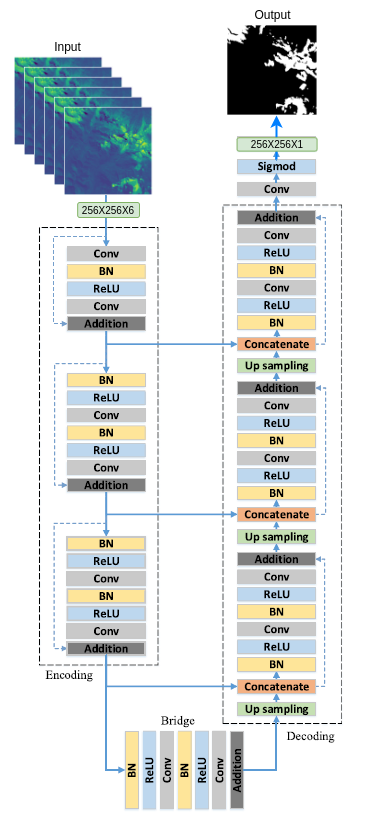
\includegraphics[width=0.5\linewidth]{graficos/RESUNET_Arquitectura}
	\caption[Arquitectura del modelo DeepResUnet.]{Arquitectura del modelo DeepResUnet.
		
	
	}
	\label{fig:RESUNET_Arquitectura}
\end{figure}

\begin{figure}[h!]
	\centering
	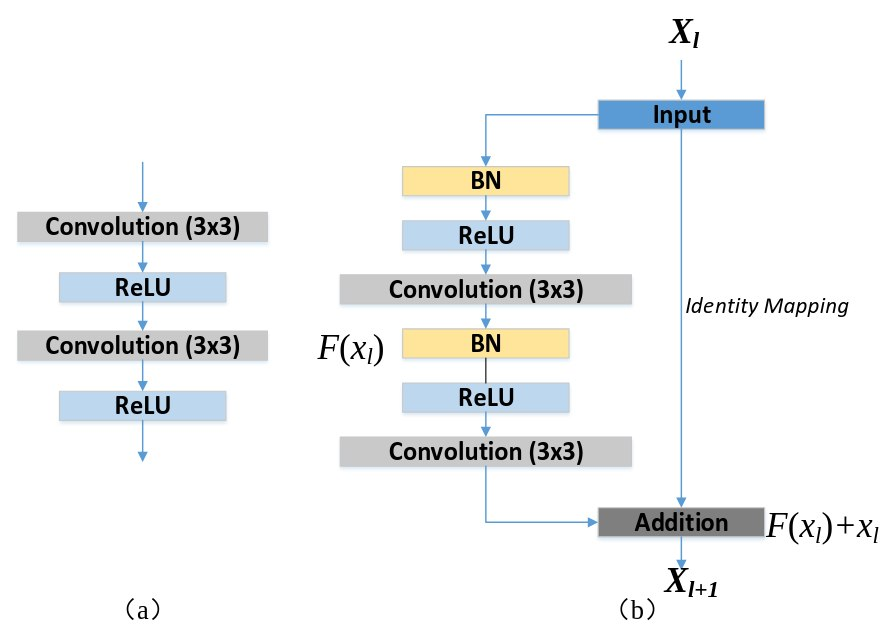
\includegraphics[width=0.7\linewidth]{graficos/residual}
	\caption[Bloques fundamentales de las redes neuronales.]{Bloques fundamentales de las redes neuronales. (a) Unidad neuronal simple utilizada en U-Net y (b) unidad residual con mapeo de identidad utilizada en el ResUnet propuesto.
		
	
	}
	\label{fig:residual}
\end{figure}




\begin{figure}[h!]
	\centering
	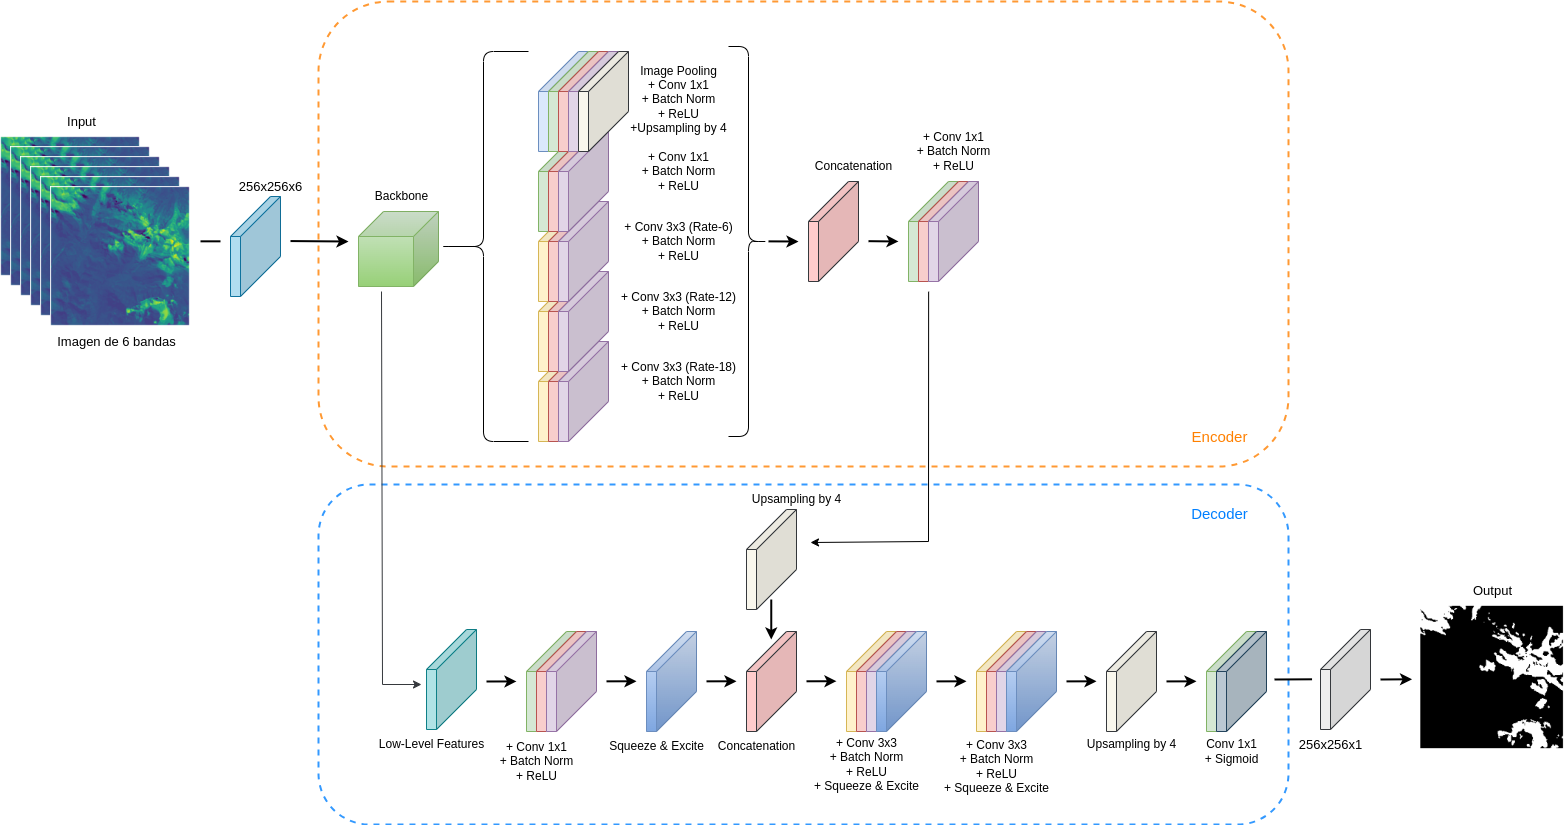
\includegraphics[width=0.9\linewidth]{graficos/DeepLabv3plusArquitectura}
	\caption[Arquitectura del modelo DeepLabV3Plus.]{Arquitectura del modelo DeepLabV3Plus.
		
	
	}
	\label{fig:DeepLabv3plusArquitectura}
\end{figure}

\subsubsection{Función de pérdida}
La función de pérdida utilizada para entrenar los modelos es una combinación ponderada de DICE Loss y BCE Loss (Binary Cross Entropy Loss), ya que ha demostrado obtener buenos resultados según \parencite{montazerolghaem2023}. La razón detrás de combinar pérdidas como DICE Loss y BCE Loss es que cada una de ellas tiene sus propias ventajas y desventajas.

\textbf{DICE Loss: } Esta pérdida es especialmente útil para tareas de segmentación donde el tamaño de la región objetivo puede ser pequeño en comparación con el fondo. Maximiza el solapamiento entre la predicción y la verdad del terreno, lo que ayuda a lidiar con el desequilibrio de clases, es decir, cuando hay muchos más píxeles de fondo que de objeto en la imagen.  

\textbf{BCE Loss: } Esta pérdida es una opción clásica para problemas de clasificación binaria, incluido cada píxel en una tarea de segmentación binaria. BCE mide la disimilitud entre las predicciones y las etiquetas verdaderas para cada píxel individualmente. Sin embargo, puede ser sensible al desequilibrio de clases.

Combinar ambas pérdidas permite aprovechar sus fortalezas individuales: BCE Loss puede proporcionar una señal de retroalimentación estable para píxeles individuales, mientras que DICE Loss puede ayudar a mejorar la predicción de los bordes del objeto y a manejar mejor el desequilibrio de clases.

\textbf{Definición Matemática de la Combinación Ponderada}

En la literatura, la combinación ponderada de funciones de pérdida se define típicamente como:

\begin{equation}
	\text{Loss} = \alpha \cdot \text{DICE Loss} + \beta \cdot \text{BCE Loss}
\end{equation}

Donde:

$\alpha$ y $\beta $ son hiperparámetros que determinan el peso de cada término de pérdida en la combinación total.
Generalmente $\alpha$ + $\beta $ = 1, pero no necesariamente. Se pueden ajustar estos párametros según cómo se requiera influir en cada termino en el entrenamiento. 

\subsubsection{Métricas de evaluación}

%%\textbf{Metricas de evaluación}

Para evaluar los modelos de segmentación semántica generados por la CNN, se utilizaron diversas métricas de evaluación: MIoU (Mean Intersection Over Union), PA (Pixel Accuracy) y Dice Coefficient (Dice).

El MIoU, definido en la ecuación~\ref{eq:miou}, se utiliza como métrica estándar en aplicaciones de segmentación para medir la superposición promedio entre las áreas predichas y las áreas reales de todas las clases.

La PA, como se muestra en la ecuación~\ref{eq:pixel_accuracy}, mide la proporción de píxeles correctamente clasificados en la imagen. Se calcula dividiendo el número de píxeles correctamente clasificados por el número total de píxeles en la imagen, proporcionando así una medida general de la precisión del modelo.

El Dice Coefficient, definido en la ecuación~\ref{eq:dice_coefficient}, evalúa la similitud entre dos conjuntos, permitiendo comparar la superposición entre una máscara de predicción y una máscara de referencia. Su valor varía entre 0 (sin coincidencias) y 1 (coincidencia perfecta), ofreciendo una medida de la precisión en la segmentación de áreas de interés.

En estas métricas, TP representa verdaderos positivos, TN indica verdaderos negativos, FP representa falsos positivos y FN señala falsos negativos.

% Fórmula para mIoU
\begin{equation}
	\label{eq:miou}
	\text{MIoU} = \frac{1}{k+1} \sum_{i=0}^{N} \frac{TP}{TP+FP+FN}
\end{equation}

% Fórmula para Pixel Accuracy
\begin{equation}
	\label{eq:pixel_accuracy}
	\text{Pixel Accuracy} = \frac{TP+TN}{TP+TN+FP+FN}
\end{equation}

% Fórmula para Dice Coefficient
\begin{equation}
	\label{eq:dice_coefficient}
	\text{Dice Coefficient} = \frac{2 \times TP}{2 \times TP+FP+FN}
\end{equation}


\subsubsection{Proceso de entrenamiento}

La plataforma computacional utilizada para implementar todos los modelos de segmentación semántica, incluyendo U-Net, ResUnet y DeepLabV3+, fue Python 3.11. Todos los marcos de aprendizaje profundo se desarrollaron utilizando el framework PyTorch 2.2.2, ejecutado sobre un sistema operativo Manjaro KDE/Linux. El hardware utilizado incluyó un procesador Intel Xeon y una GPU NVIDIA Quadro P2000 con 5 GB de memoria.

\begin{figure}[h!]
	\centering
	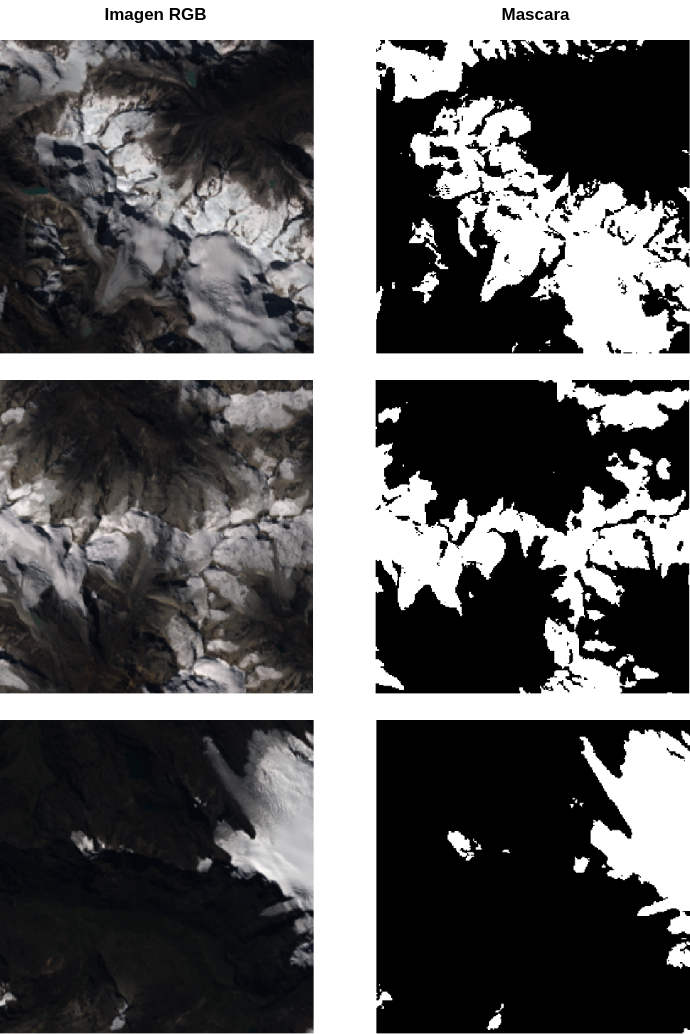
\includegraphics[width=0.7\linewidth]{graficos/rgb_mascara}
	\caption[Representación de muestras de conjuntos de datos (RGB y máscara) utilizadas para entrenar el modelo.]{Representación de muestras de conjuntos de datos segmentados de diferentes ubicaciones (RGB y su respectiva máscara) utilizadas para entrenar los modelos propuestos.
		
	}
	\label{fig:rgb_mascara}
\end{figure}





Durante esta etapa, se llevó a cabo el entrenamiento de las tres arquitecturas de segmentación semántica propuestas. Se realizaron numerosos experimentos para identificar los parámetros óptimos de entrenamiento, tales como el optimizador, el número de épocas, la tasa de aprendizaje, el tamaño del batch, el número de trabajadores (num workers) y el factor de decaimiento de los pesos (weight decay). La selección cuidadosa de estos parámetros fue esencial para garantizar que los modelos convergieran de manera eficiente y alcanzaran los mejores pesos posibles. Esta optimización no solo maximiza el rendimiento de la red neuronal, sino que también mejora su capacidad para generalizar de manera efectiva a través de diferentes conjuntos de datos. Además, se evaluó el impacto de estos parámetros en la precisión y robustez de los modelos, asegurando que el proceso de entrenamiento resultara en una segmentación precisa y confiable.

Siguiendo las recomendaciones de la documentación de PyTorch \parencite{pytorch-lr-scheduler}, se utilizó el método "ReduceLROnPlateau" para ajustar dinámicamente la tasa de aprendizaje cuando una métrica de rendimiento dejaba de mejorar. Este enfoque es particularmente beneficioso, ya que la reducción de la tasa de aprendizaje en un factor de 2 a 10 puede ayudar a superar estancamientos durante el entrenamiento. En este contexto, el algoritmo monitoreó continuamente las métricas de evaluación y, si no se observaba ninguna mejora en un periodo de 5 épocas consecutivas, automáticamente reducía la tasa de aprendizaje. Esta estrategia permite que el modelo ajuste su proceso de aprendizaje de manera más refinada, optimizando así su capacidad para converger a una solución óptima.


Finalmente, para contar con un amplio conjunto de datos se realizó un data augmentation para evitar el sobreajuste del modelo, se aplicó rotaciones de $90^\circ$ y reflejo de espejo horizontal y vertical a la imagen multiespectral de 6 canales y sus respectivas máscaras.
 
%% CHATgpt : U-NET ARQUITECTURE OVERVIEW


\begin{table}[h!]
	\centering
	\begin{tabular}{|c|c|c|c|c|c|c|}
		\hline
		\textbf{Modelo} & \textbf{Optimizer} & \textbf{Epochs} & \textbf{Learning rate} & \textbf{Batch size} & \textbf{num workers} & \textbf{weight decay}\\
		\hline
		U-Net  & Adam & 25 & 1e-3 & 4 & 8 & 1e-2 \\
		ResUnet   & Adam & 25 & 1e-3 & 4 & 8 & 1e-2 \\
		DeepLabV3+ & Adam & 25  & 1e-4 & 4 & 8 & 1e-6 \\
		
		\hline
	\end{tabular}
	\caption{Párametros de entrenamiento}
	\label{tabla2}
\end{table}

%\section{Experimentos y resultados}
\subsection{Resultados de entrenamiento}

%Los modelos de CNN propuestos se entrenaron en 30 épocas de acuerdo con los gráficos de precisión y pérdida de entrenamiento/validación como se muestra en la graficas  \ref{fig:training_metric_U_NET2}, \ref{fig:training_metric_RESUNET} y \ref{fig:training_metric_DeepLabV3}. Para lograr el mejor rendimiento y estabilidad del entrenamiento, asumimos que todos los modelos fueron entrenados bien de acuerdo con los valores de hiperparametros mejor optimizados enumerados en la tabla ~\ref{tabla2}. Los mejores valores de hiperparametros se lograron entrenando varios modelos basados en diferentes valores de hiperparametros para lograr el mejor rendimiento del modelo y estabilidad del entrenamiento. Los modelos entrenados se evaluaron utilizando un conjunto de datos de prueba para evaluar el rendimiento de los modelos propuestos en función a las metricas escritas en las ecuaciones ~\ref{eq:miou} - ~\ref{eq:dice_coefficient}.


Los modelos de redes neuronales convolucionales (CNN) propuestos fueron entrenados durante 25 épocas, guiados por los gráficos de precisión y pérdida tanto en el entrenamiento como en la validación, como se ilustra en las figuras \ref{fig:training_metric_U_NET2}, \ref{fig:training_metric_RESUNET} y \ref{fig:training_metric_DeepLabV3}. Para asegurar un rendimiento óptimo y estabilidad en el proceso de entrenamiento, se asumió que todos los modelos se entrenaron correctamente siguiendo los valores de hiperparámetros óptimos, los cuales se encuentran detallados en la tabla \ref{tabla2}. Estos valores de hiperparámetros fueron seleccionados después de entrenar múltiples veces los modelos con diferentes configuraciones, con el objetivo de encontrar la combinación que ofreciera el mejor desempeño y estabilidad.

%Una vez entrenados, los modelos fueron evaluados utilizando un conjunto de datos de prueba para medir su rendimiento en términos de las métricas descritas en las ecuaciones \ref{eq:miou} - \ref{eq:dice_coefficient}. Esta evaluación permitió comprobar la efectividad de los modelos propuestos, asegurando que los resultados obtenidos fueran representativos de su capacidad para generalizar y segmentar adecuadamente en diferentes escenarios.

\begin{figure}[h!]
	\centering
	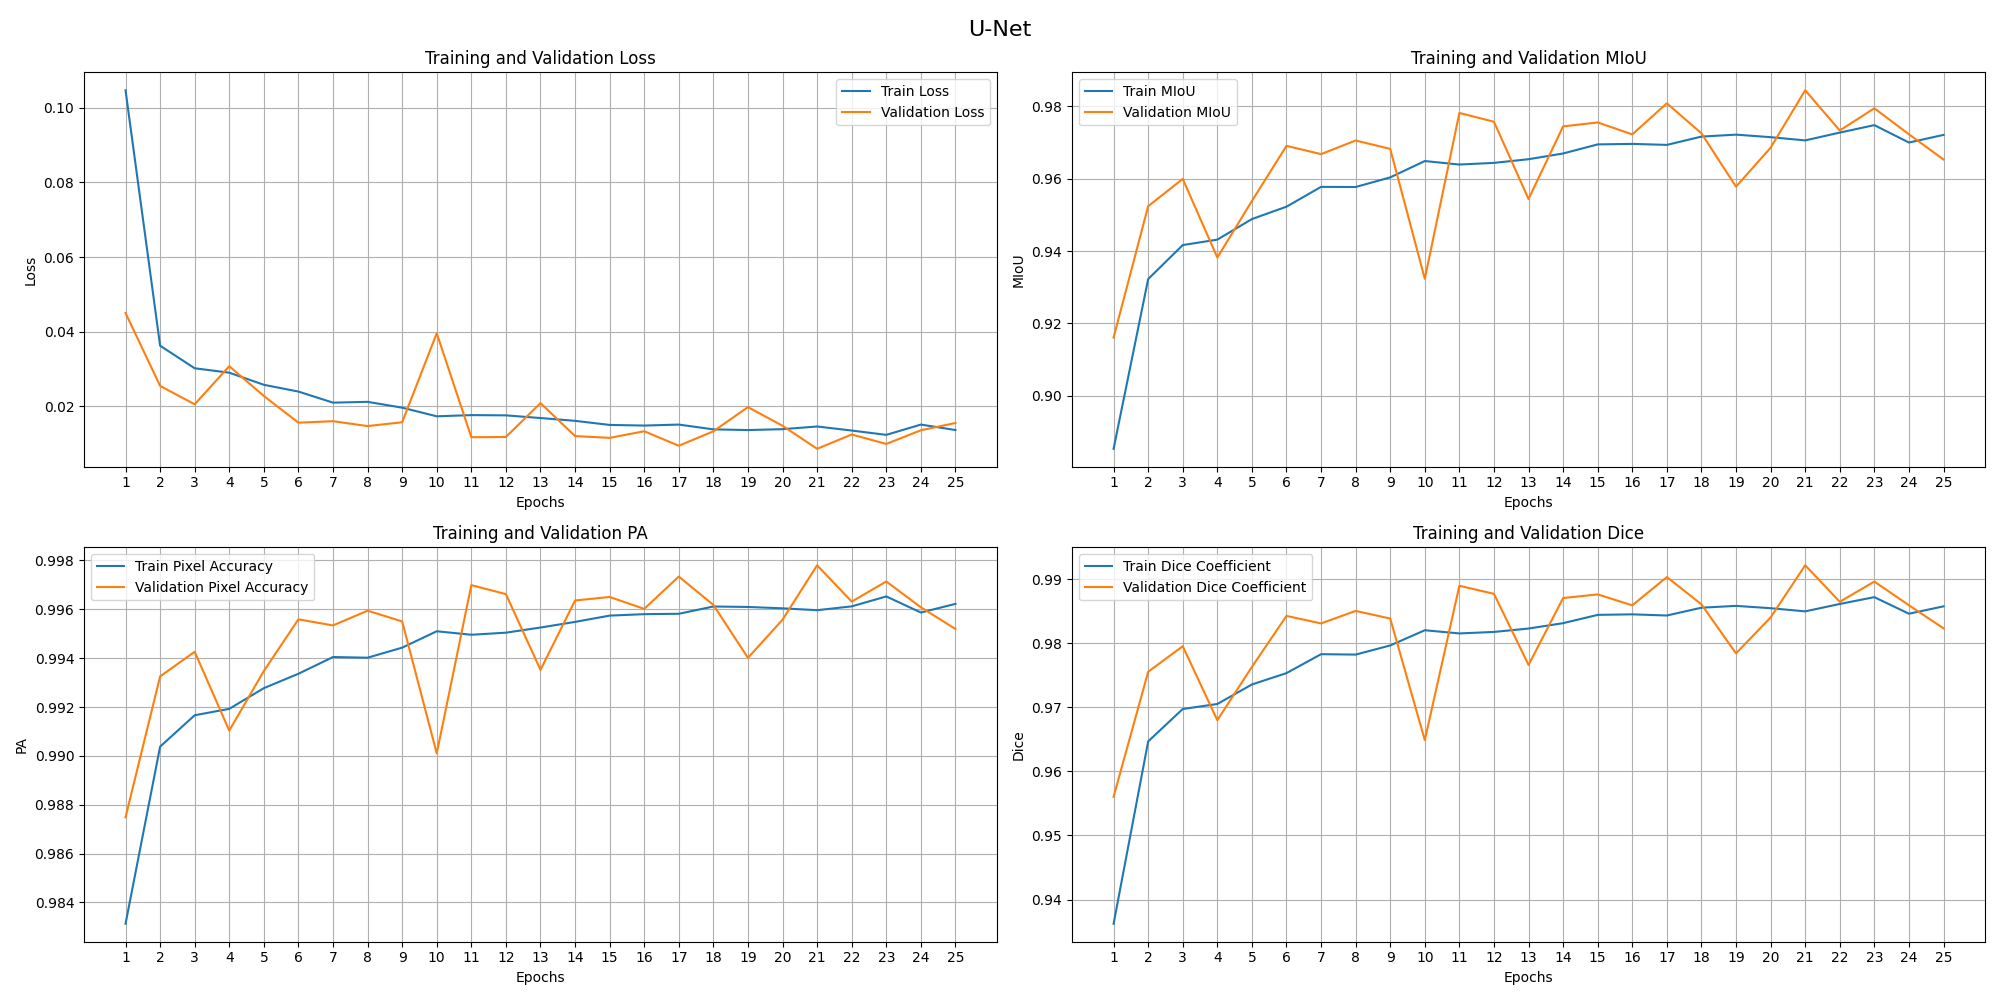
\includegraphics[width=\linewidth]{graficos/training_metric_Unet_L5_L8_C2L1_P1}
	\caption[Gráficos de pérdida de entrenamiento y métricas de precisión para U-NET.]{Gráficos de pérdida de entrenamiento y métricas de precisión para U-NET.
		
	}
	\label{fig:training_metric_U_NET2}
\end{figure}


\begin{figure}[h!]
	\centering
	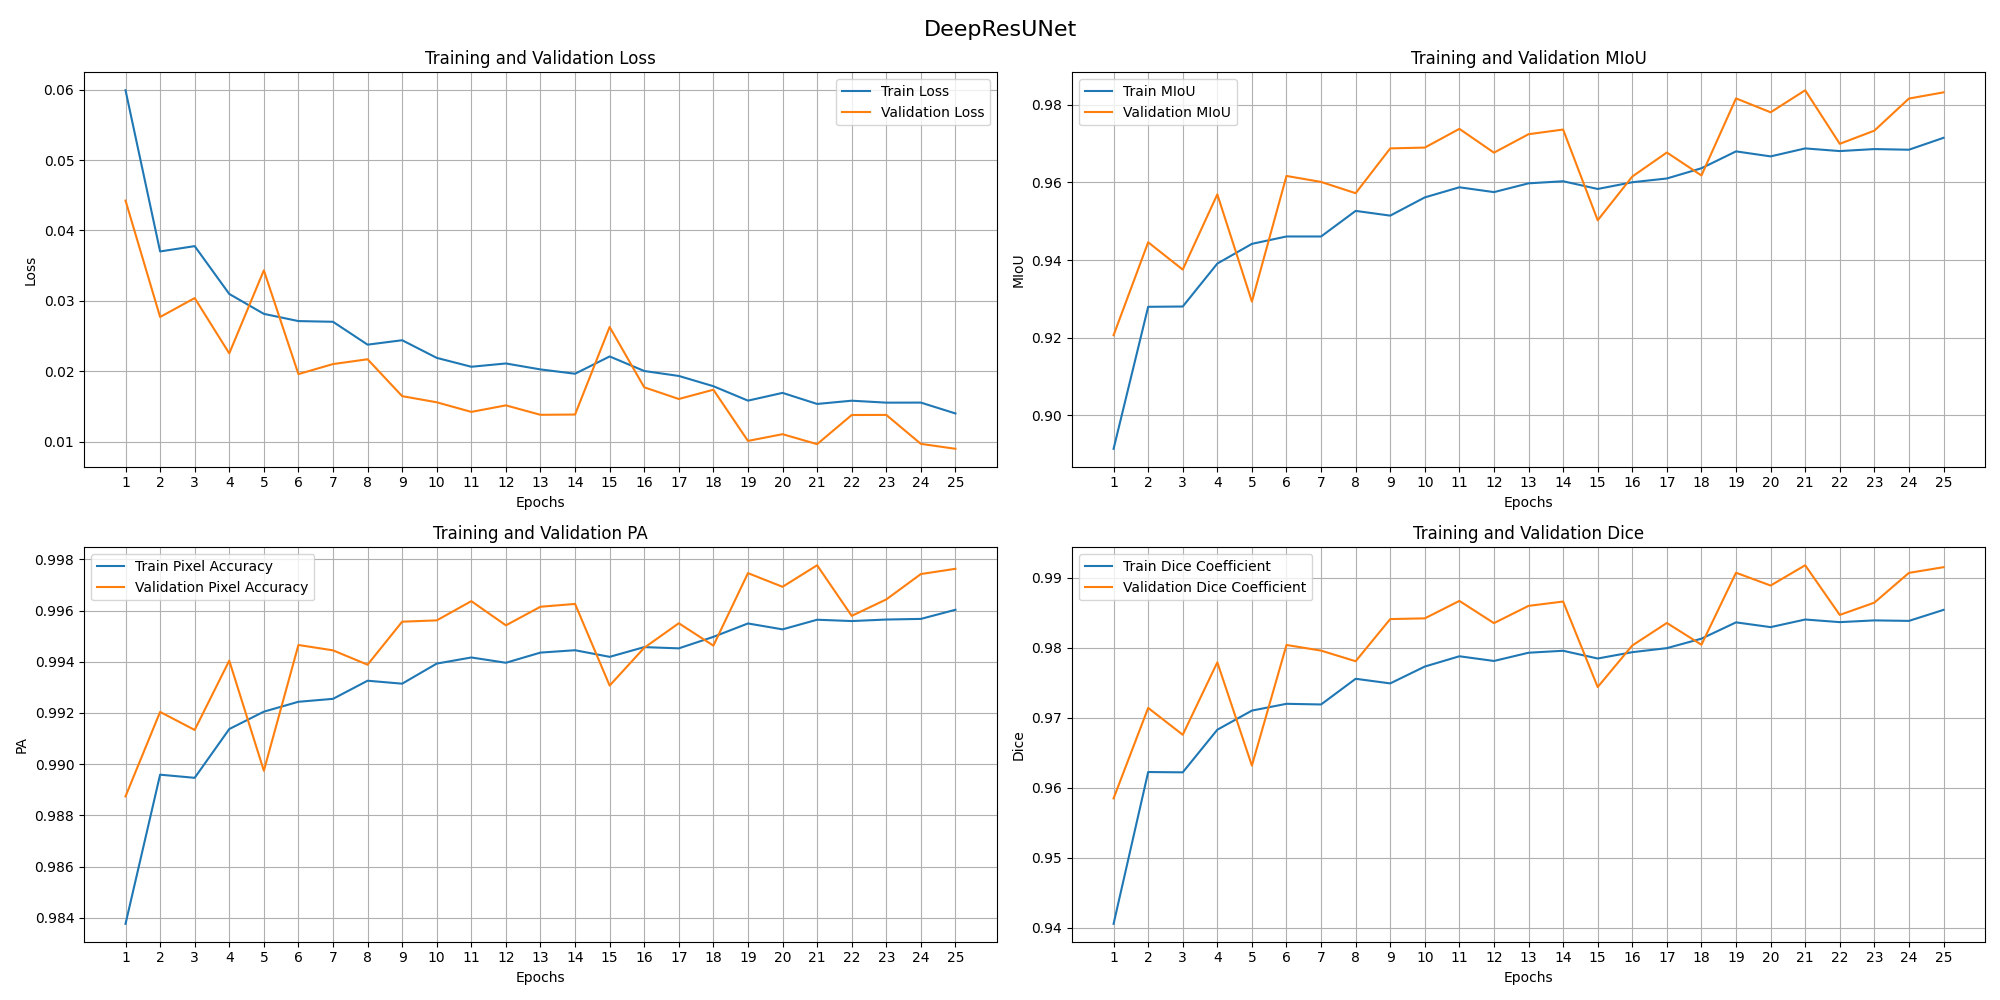
\includegraphics[width=\linewidth]{graficos/training_metric_DeepResUnet_L5_L8_C2L1_P1}
	\caption[Gráficos de pérdida de entrenamiento y métricas de precisión para DeepResUnet.]{Gráficos de pérdida de entrenamiento y métricas de precisión para RESUNET.
		
		
	}
	\label{fig:training_metric_RESUNET}
\end{figure}


\begin{figure}[h!]
	\centering
	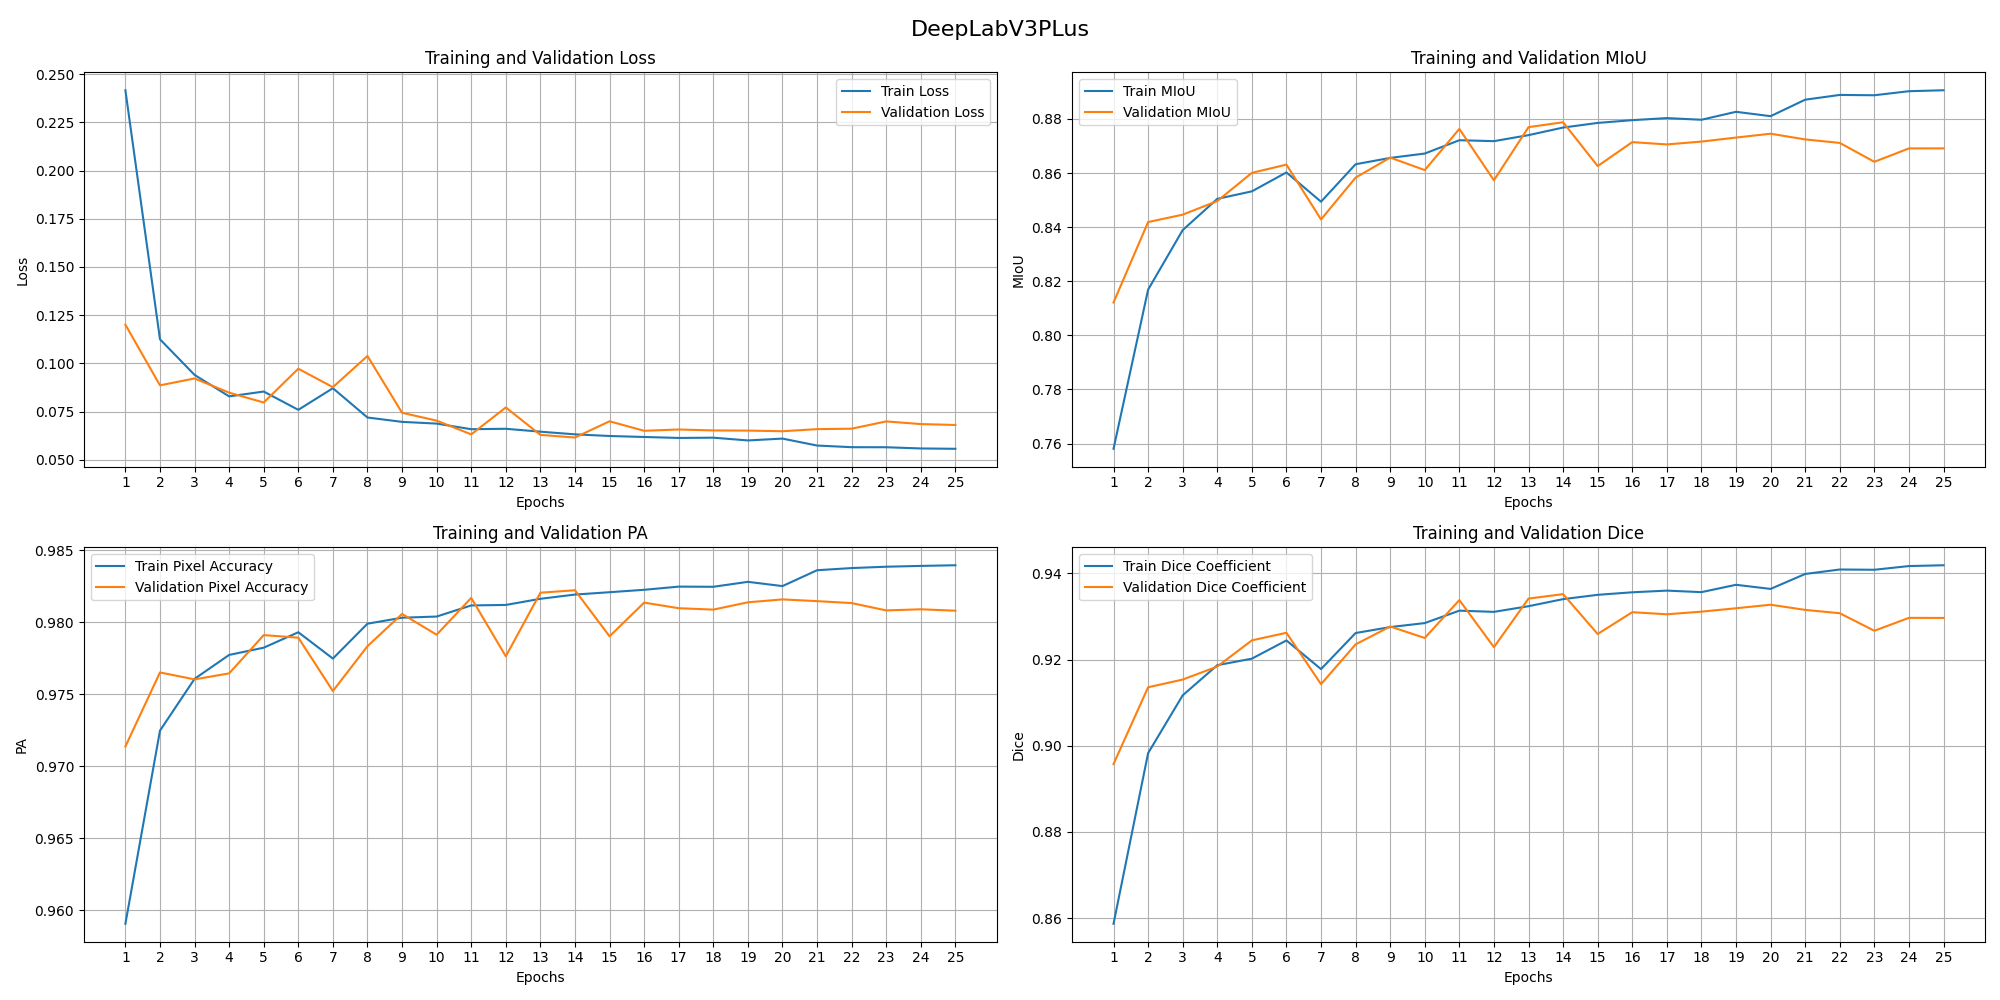
\includegraphics[width=\linewidth]{graficos/training_metric_DeepLabV3PLus_L5_L8_C2L1_P1}
	\caption[Gráficos de pérdida de entrenamiento y métricas de precisión para DeepLabV3Plus.]{Gráficos de pérdida de entrenamiento y métricas de precisión para DeepLabV3Plus.
		
		
	}
	\label{fig:training_metric_DeepLabV3}
\end{figure}


%En las Figuras \ref{fig:Miou_vs_epochs}, \ref{fig:PA_vs_epochs} y \ref{fig:DICE_vs_epochs}, se muestran los resultados de las métricas MIoU (Mean Intersection over Union), PA (Pixel Accuracy) y Dice Coefficient (Dice) evaluadas para cada modelo CNN utilizando los datos de evaluación. 


%Los gráficos revelan que U-Net y DeepResUnet presentan un comportamiento muy similar y consistente, lo cual indica que estas redes realizan un proceso de segmentación semántica eficiente. Sin embargo, los resultados del modelo DeeplabV3Plus no son alentadores, ya que no alcanza un desempeño competitivo frente a U-Net y DeepResUnet.


%En la Figura \ref{fig:Loss_vs_epochs} se muestran los resultados del comportamiento de la función de pérdida para cada modelo utilizando los datos de evaluación. Se observa que la función de pérdida converge de manera más efectiva en los modelos U-Net y DeepResUnet, mientras que en el caso de DeepLabV3Plus, esta función de pérdida permanece elevada en comparación con U-Net y DeepResUnet.


%\subsection{Resultado}

%Los modelos fueron evaluados utilizando un conjunto de datos de evaluación 1200 imágenes de prueba, evaluando la presición utilizando las metricas mIoU, Dicce Coefccient y PA, en la tabla ~\ref{tabla3} se muestran las metricas cuantitativas. Basandonos en la integración de las bandas 2,3,4,5,6 y 7 de Landsat 8 Collection 2 Level-2, ResUNet logra tener las metricas más adecuadas y el mejor rendimiento al clasificar y segmentar con muy buena precisión la información de limites de una amplia gama de glaciares, pero tiene el mas alto numero de parametros de entrenamiento en comparación con U-Net y DeepLabV3+, esto se debe al mecanismo residual, que causa un alto costo computacional. 


\begin{comment}


La Figura \ref{fig:comparative_predictions} muestra los resultados de segmentación obtenidos por los modelos propuestos. DeepLabV3Plus no logró segmentar los cuerpos glaciares con suficiente detalle, aunque presentó un comportamiento aceptable en general. Por su parte, el modelo DeepResUnet logró segmentar los límites de los cuerpos glaciares de manera más completa, mostrando un rendimiento superior en comparación con DeepLabV3+. Sin embargo, el mejor desempeño fue alcanzado por U-Net, que ofreció una segmentación más precisa y exacta de los límites glaciares, reflejando su capacidad para capturar detalles con mayor fidelidad.


\begin{figure}[h!]
	\centering
	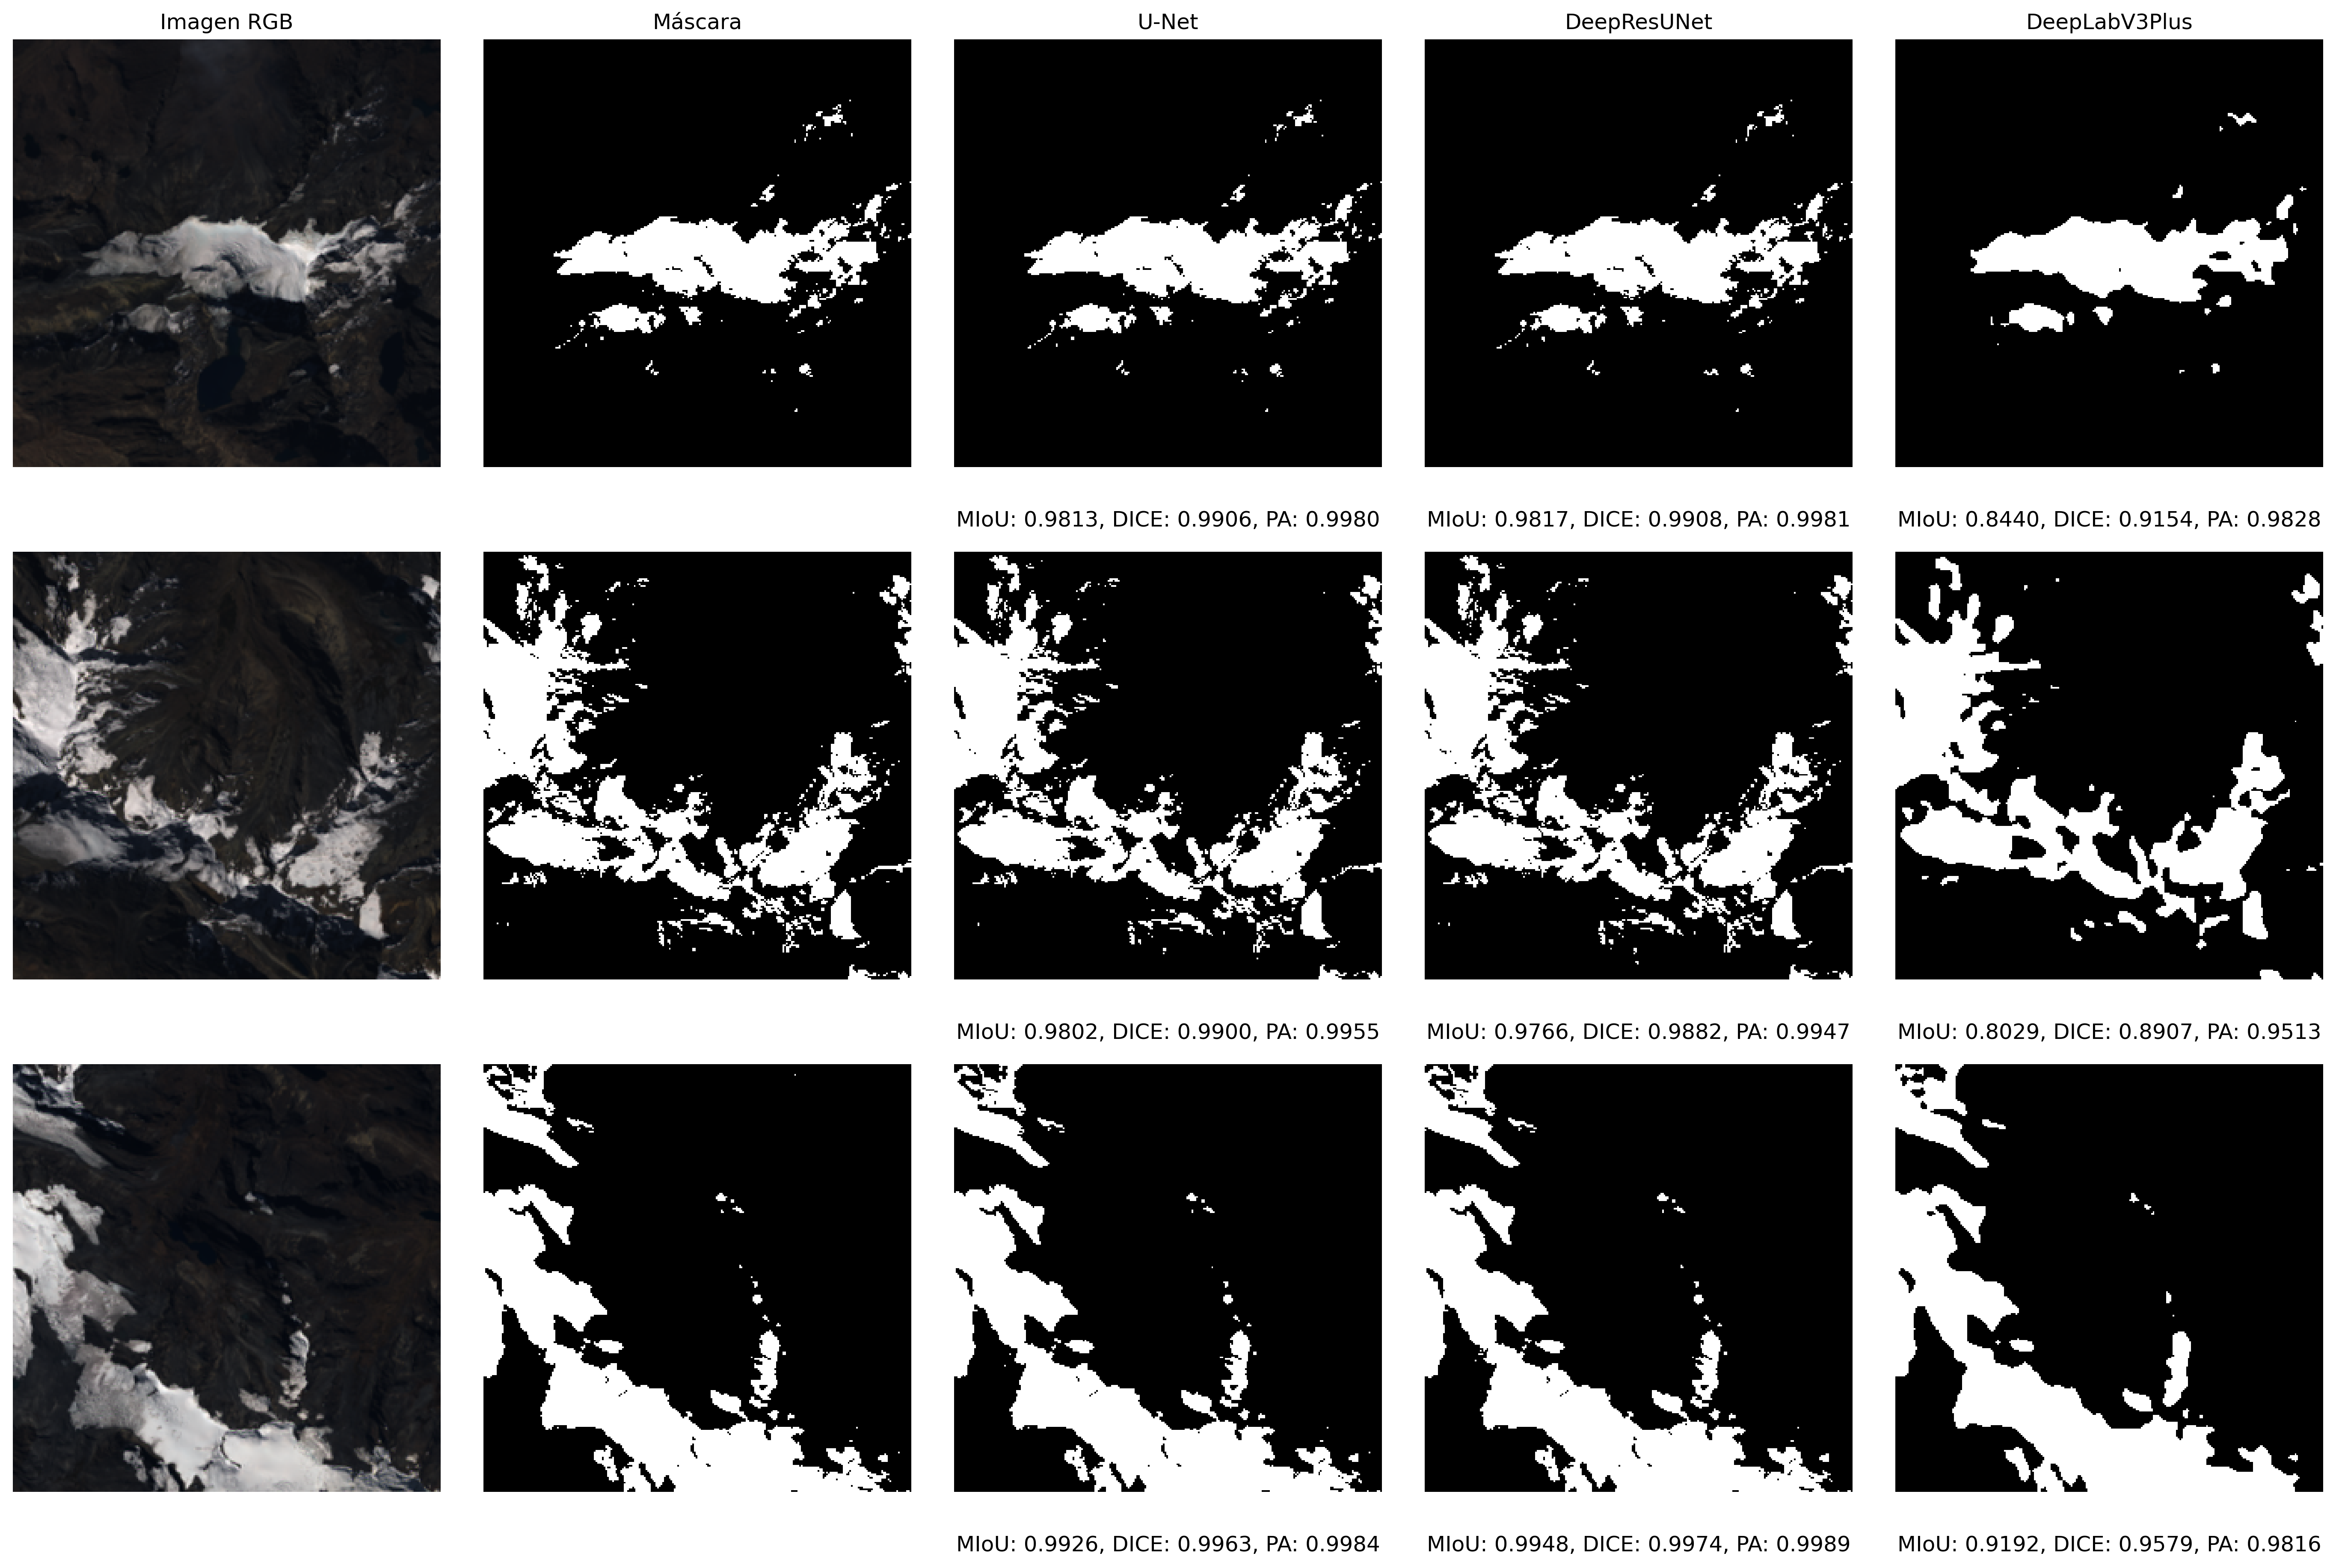
\includegraphics[width=0.7\linewidth]{graficos/comparative_predictions}
	\caption[Análisis cualitativo y cuantitativo de los modelos eveluados.]{Cualitativamente, tanto U-Net como ResUnet muestran una gran similitud con las máscaras de referencia, logrando segmentar con precisión los bordes de los cuerpos glaciares. En contraste, aunque DeepLabV3Plus logra una segmentación aceptable, no alcanza el mismo nivel de precisión en la delimitación de los bordes.
		Cuantitativamente, U-Net muestra un rendimiento sobresaliente, mientras que DeepResUnet ofrece un rendimiento competitivo. En comparación, DeepLabV3Plus no alcanza un nivel competitivo frente a los otros modelos.
		
	}
	\label{fig:comparative_predictions}
\end{figure}




El enfoque utilizado para el análisis temporal, con el fin de reducir la influencia de la nieve efímera, consistió en analizar múltiples escenas durante la estación seca y seleccionar aquellas que mejor representaran la extensión del glaciar. Para ello, se eligieron únicamente escenas sin nieve efímera visible en el paisaje circundante al glaciar, aplicando una técnica de preselección común.

Posteriormente, se creó un conjunto de datos que incluye únicamente las imágenes del glaciar Quelccaya, seleccionando las más representativas de los años de interés. Este dataset fue preprocesado y utilizado como entrada para la red neuronal U-Net, con el objetivo de generar imágenes predichas que luego se emplearían para calcular el área del glaciar en cada año.

Dado que la red neuronal acepta entradas de tamaño 256x256, fue necesario reconstruir las imágenes predichas a un tamaño de 512x512, adecuado para contener la totalidad del glaciar Quelccaya. Una vez reconstruida, la imagen resultante es completamente binaria, con un tamaño de 512x512, donde los píxeles blancos segmentados representan los cuerpos glaciares y los píxeles negros cualquier otra superficie.

Cada imagen binaria se procesa sumando los píxeles blancos, considerando que cada píxel tiene una resolución de 30 metros. De esta manera, se calcula el área del glaciar correspondiente a cada año. Este procedimiento se repite para los demás años de interés.


\begin{figure}[h!]
	\centering
	\includegraphics[width=0.7\linewidth]{graficos/reconstruir_imagen}
	\caption[Proceso de predicción y reconstrucción para calcular el área segmentada.]{Proceso de predicción y reconstrucción para calcular el área segmentada.
		
	}
	\label{fig:reconstruir_imagen}
\end{figure}

En la figura \ref{fig:predicciones_temporales}, se visualizan los cambios en la superficie del glaciar Quelccaya para los años 1991, 2006 y 2024, con el propósito de proporcionar una mejor representación del retroceso glaciar. En esta figura se muestran los bordes correspondientes a cada año: el borde azul indica la extensión del glaciar en 1991, el borde rojo en 2006 y el borde rosado en 2024. Se observa claramente un retroceso significativo en la superficie glaciar a lo largo del tiempo, siendo más pronunciado en el lado occidental del glaciar en comparación con el lado oriental. Además, conforme el área glaciar ha disminuido, se ha evidenciado la formación y expansión de varias lagunas en la zona.

\begin{figure}[h]
	\centering
	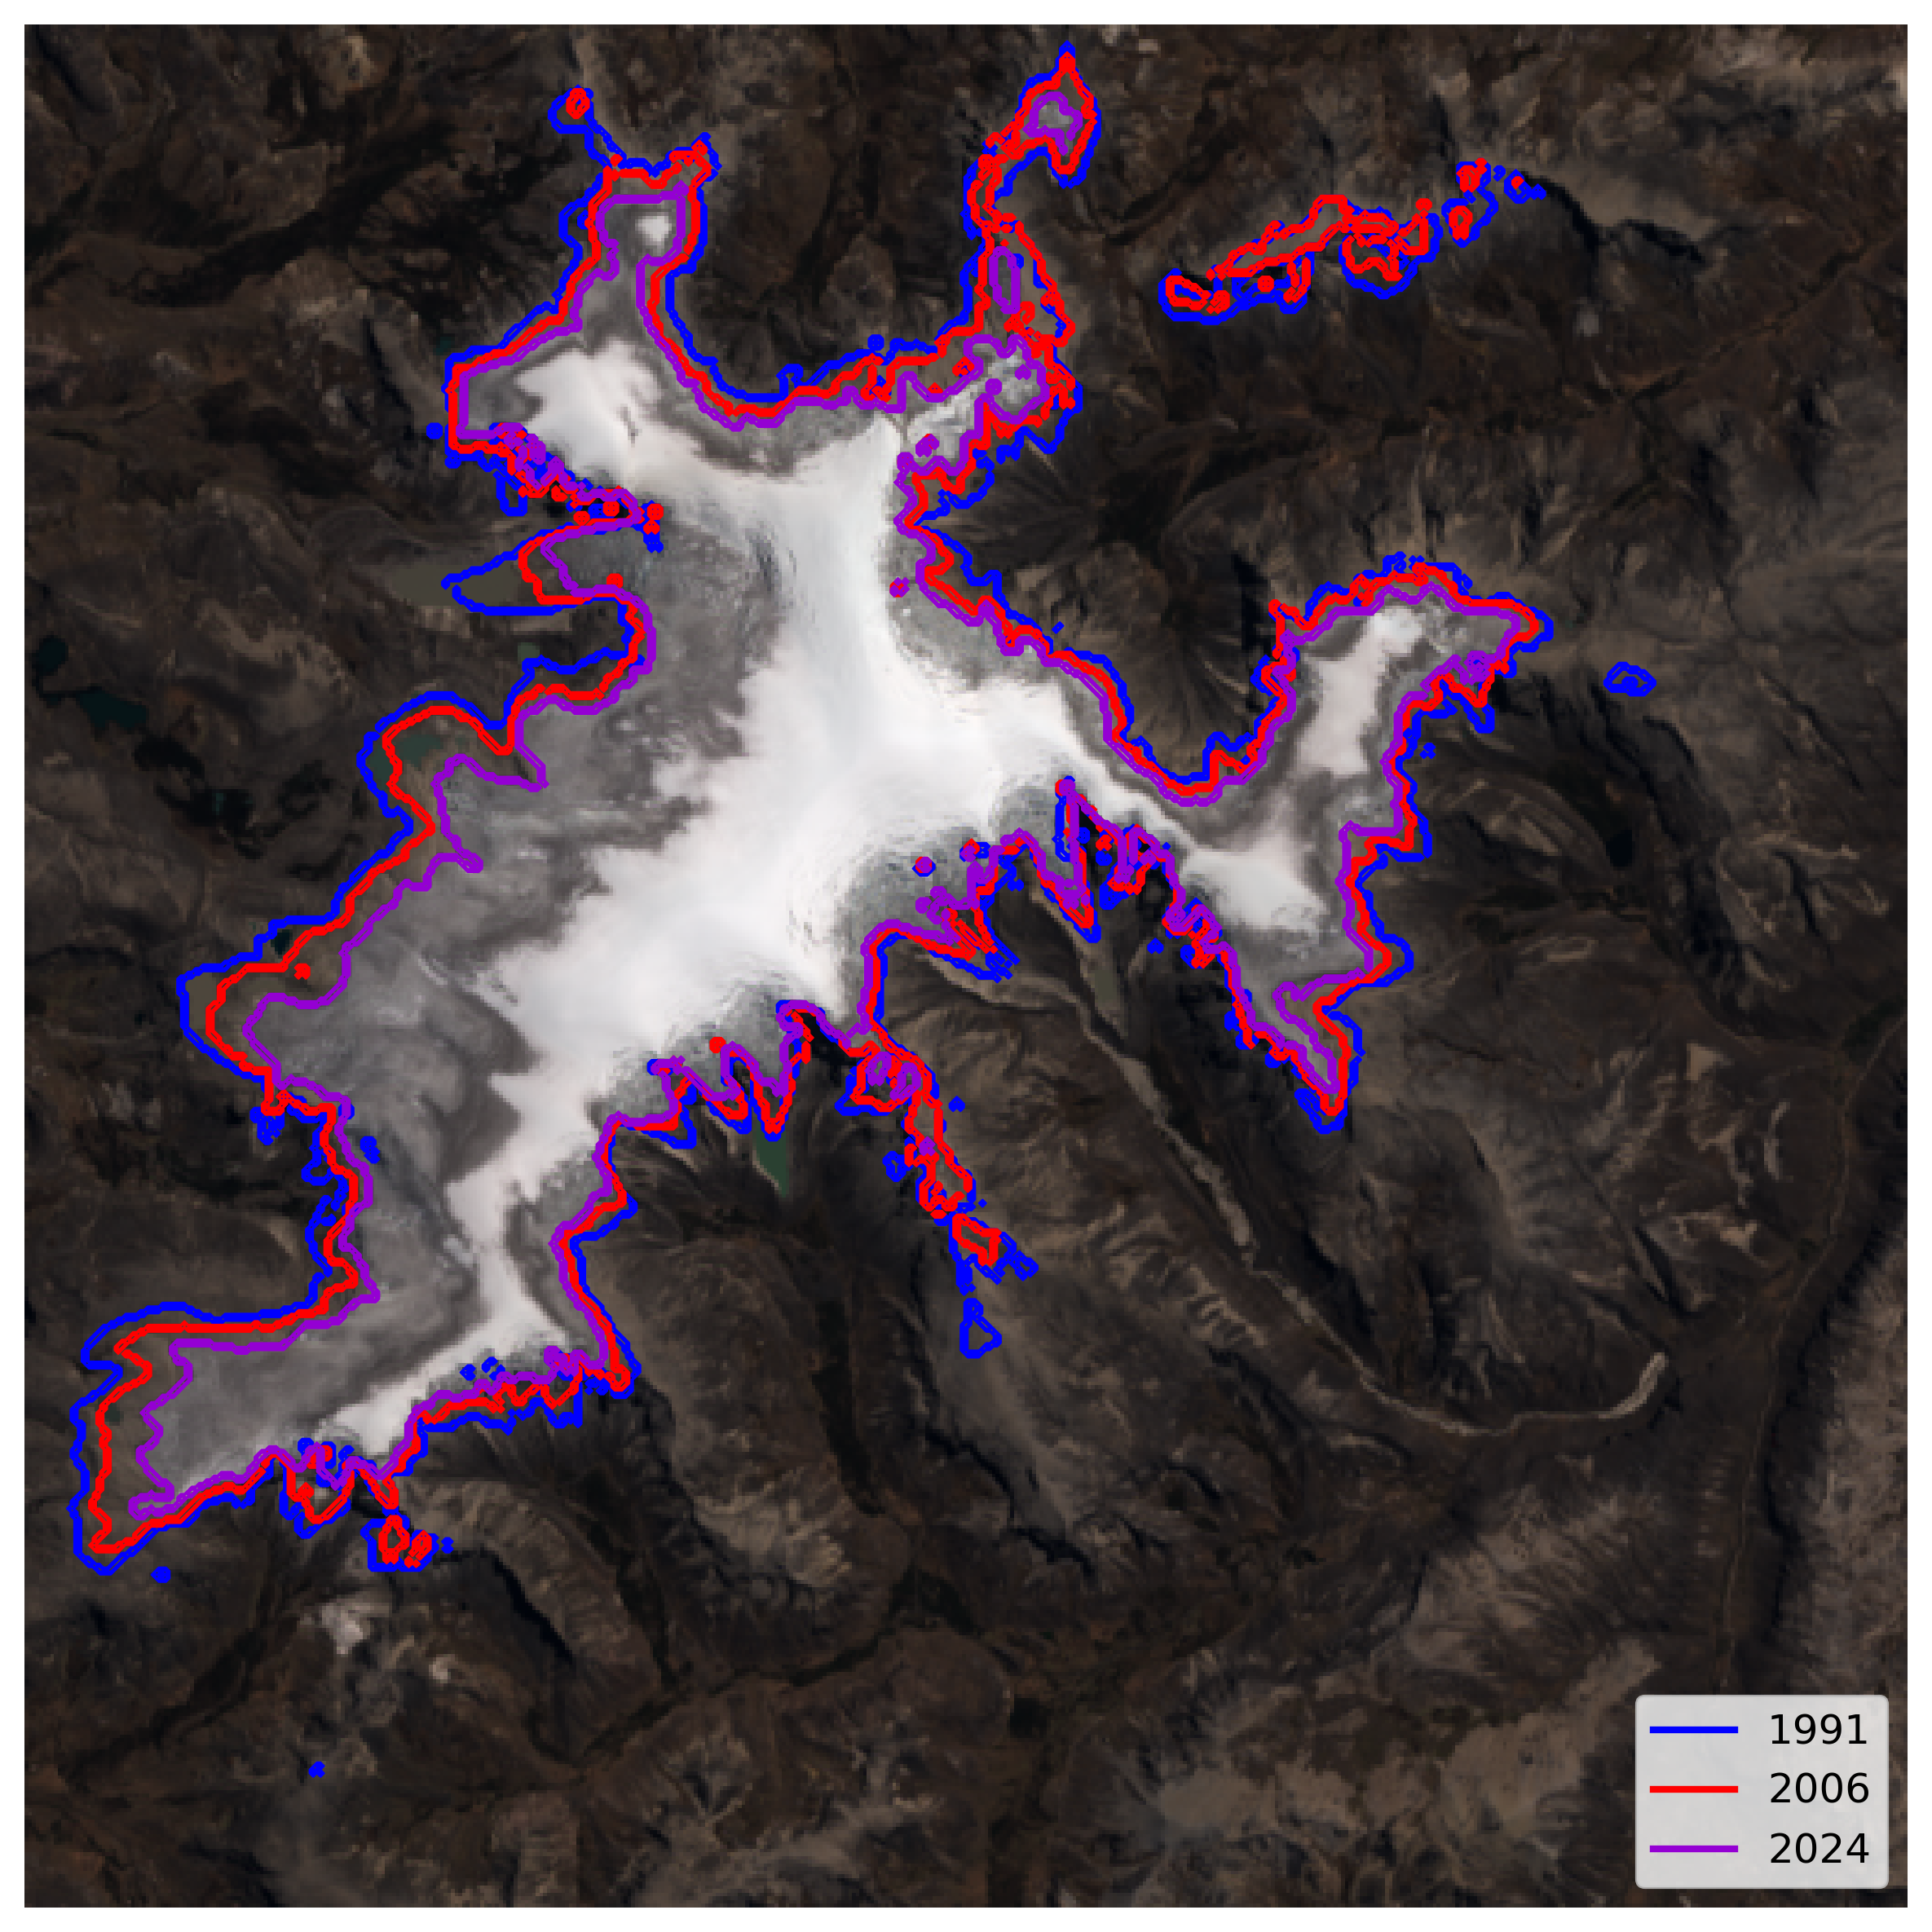
\includegraphics[width=0.7\linewidth]{graficos/predicciones_temporales}
	\caption[Contornos glaciares más antiguos y mas recientes del Glaciar Quelccaya.]{Contornos glaciares más antiguos y mas recientes del Glaciar Quelccaya.
		
	}
	\label{fig:predicciones_temporales}
\end{figure}
 





%Se ha realizado una gráfica de la serie temporal tal como se muestra en la figura, para cuantificar el retroceso glaciar. Los resultados indican que la superficie del glaciar Quelccaya ha disminuido notablemente en un 30.15\% durante el periodo 1991-2024, pasando de 50.81 km² en 1991 a 35.49 km² en 2024. Esto representa una tasa de disminución de 0.424 ± 0.136 km²/año, con todas las incertidumbres expresadas como intervalos de confianza del 95 \%.En el análisis se excluyeron algunos años, ya que se comprobó que no representaban con precisión la extensión de la capa de hielo. Estos años mostraban áreas anómalas, probablemente debido a la presencia de nieve efímera, una fuente potencialmente significativa de inexactitud al analizar escenas con esta cobertura temporal.

%\subsection{Comparación con trabajos previos}

%Los antecedentes sobre estimulación del area del glacear Quelccaya son muy escasas la mayoria de los estudios limitan su analisis a estudiar regiones mucho mas amplia. Ademas los limites glaciares analizados no son fijos, puesto que en la mayoria de los casos los autores suelen elegir manualmente las imagens satelitales que podrian no contener nieve temporal para evitar resultados inadecuados, para comparar los resultados obtenidos de esta investigación se concidera los estudios realizados por \parencite{malone2022evolution}, \parencite{taylor2022multi} y \parencite{hanshaw2014glacial}, donde \parencite{malone2022evolution} y \parencite{taylor2022multi} son estudios recientes que incluyen es estudio temporal del glaciar Quelccaya. Los resultados de la estimacion de áreas glacear de esta investigación para el glaciar Quelccaya llegan a tener valores muy cercanos a los antecedentes y en alghunos años el valor de área glaciar incluso fue muy proximo a los antecedentes, tal es el caso de los años 1991, 1992, 1995, 1999, 2006, 2009, 2015, 2019, 2020, En la figura se puede observar que algunos valores de área glaciar de este estudio son muy cercanos y aun logran superponerse, de igual forma hay algunos valores que son ligeramente alejados, pero en general la mayoria de los datos llegan a estar muy proximos a los antecedentes. ademas los resultados en general son mucho mas comparables y similares a los resultados de \parencite{malone2022evolution} sn embargo, suele existir discrepancias en algunos valores que probablemente se deba a la forma de trazado de limites de los glaciares, el estudio actual informa datos cuenta con datos con una resolución de 30 metros. Para Los resultados del el año 2020, año en que finaliso el analsis para \parencite{taylor2022multi} y \parencite{malone2022evolution},  se obtubo un area glaciar de  41.58 km² para \parencite{taylor2022multi}, de 39.03 km² para \parencite{malone2022evolution}  y para este estudio es de el area obtenida fue de 38.99 km², la tasa de retroceso glaciar para \parencite{malone2022evolution} fue de 0.43 km²/año, mientras que para esta investigación la tasa de retroceso glaciar es de 0.3935 km²/año, sin embargo este estudio extendio el analisis temporal hasta 2024 llegando a tener un area de 35.49 km².

\subsection{Comparación con trabajos previos}

Los antecedentes sobre la estimación del área del glaciar Quelccaya son limitados, ya que la mayoría de los estudios se han enfocado en regiones glaciares más extensas. Además, los límites glaciares utilizados en estos estudios no suelen ser consistentes, ya que los investigadores frecuentemente seleccionan manualmente las imágenes satelitales que parecen no tener nieve efímera para evitar resultados inexactos. Para comparar los resultados de esta investigación, se consideraron los estudios de \parencite{malone2022evolution}, \parencite{taylor2022multi} y \parencite{hanshaw2014glacial}. Estos estudios emplearon el método NDSI (Índice Normalizado de Diferencia de Nieve) para segmentar el glaciar Quelccaya y posteriormente estimar el área glaciar mediante un análisis temporal, usando imágenes satelitales de la serie Landsat con una resolución de 30 metros. En particular, \parencite{malone2022evolution} y \parencite{taylor2022multi} son investigaciones recientes que incluyen un análisis temporal detallado del glaciar Quelccaya.

Los resultados de la estimación de área glaciar obtenidos en este estudio presentan valores muy cercanos a los reportados en investigaciones previas. En años específicos, como 1991, 1992, 1995, 1999, 2006, 2009, 2015, 2019 y 2020, las estimaciones de área glaciar de este estudio son notablemente similares a las obtenidas en estudios anteriores. En la Figura \ref{regresion_new} correspondiente, se observa que varios de estos valores se superponen o son muy cercanos a los resultados de otros estudios, aunque también existen pequeñas discrepancias. En general, los datos de este trabajo se asemejan más a los resultados de \parencite{malone2022evolution}. Sin embargo, las diferencias menores en algunos años podrían atribuirse a variaciones en la delimitación de los bordes del glaciar o a fenómenos climáticos interanuales, como El Niño o La Niña. Cabe destacar que los datos de esta investigación cuentan con una resolución espacial de 30 metros, equivalente a la de los estudios comparados.

En cuanto a los resultados específicos, para el año 1991 (inicio del análisis temporal en este estudio), la estimación del área glaciar en \parencite{taylor2022multi} fue de 50.21 km², en \parencite{malone2022evolution} fue de 50.89 km², mientras que en este estudio fue de 50.81 km². Para el año 2020, último año de análisis en \parencite{taylor2022multi} y \parencite{malone2022evolution}, los valores de área glaciar fueron 41.58 km² en \parencite{taylor2022multi}, 39.03 km² en \parencite{malone2022evolution} y 38.99 km² en este estudio. Se observa que los resultados obtenidos en esta investigación son muy similares a los de \parencite{malone2022evolution}. La tasa de retroceso glaciar estimada por \parencite{malone2022evolution} fue de 0.43 km²/año, mientras que en este estudio se obtuvo una tasa de 0.393 km²/año. Es importante señalar que \parencite{taylor2022multi} no proporciona una tasa de retroceso específica para el glaciar Quelccaya.

Este estudio amplía el análisis temporal hasta 2024, año en el cual el área glaciar se ha reducido a 35.49 km². En la Figura \ref{regresion_new} correspondiente se pueden observar algunos años excluidos del análisis; esto se debe a que las imágenes de esos años presentaban nieve temporal o nubes, lo cual afectaría la precisión de los resultados. Además, algunas imágenes no estaban disponibles para todos los años, lo que limitó la continuidad en ciertas observaciones.

\begin{figure}[h!]
	\centering
	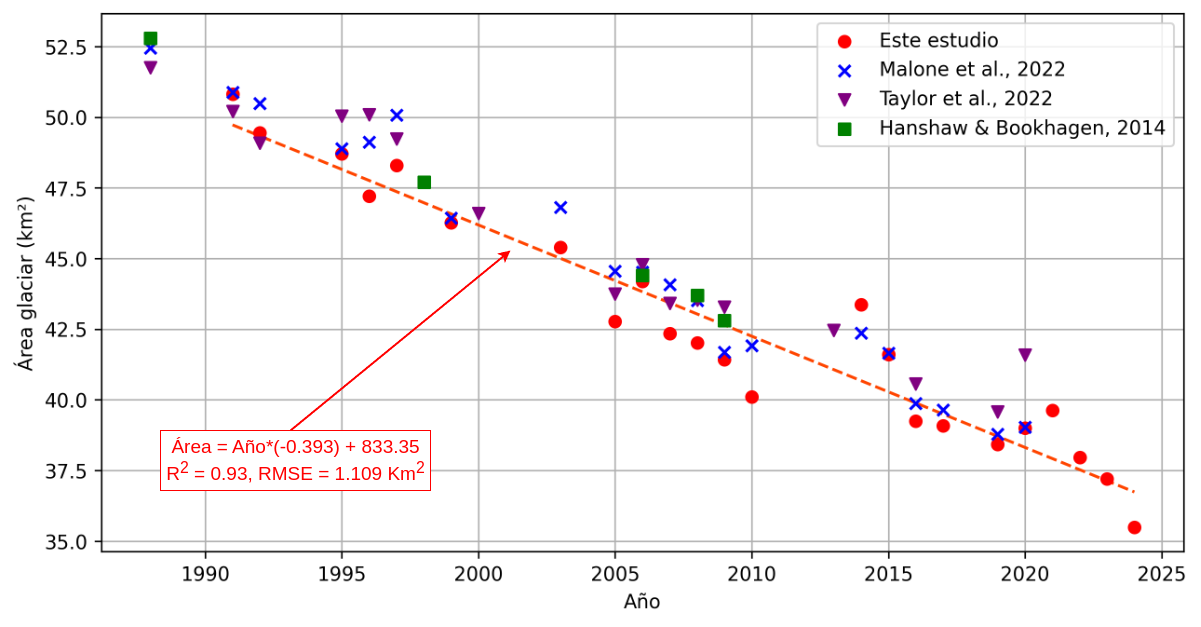
\includegraphics[width=0.9\linewidth]{graficos/regresion_new}
	\caption[Serie temporal de superficie glaciar Quelccaya.]{Serie temporal del área glaciar del Quelccaya. Los puntos rojos representan el área glaciar estimada en cada año según los resultados de este estudio, mientras que los demás símbolos corresponden a las estimaciones de estudios previos. La línea entrecortada muestra la regresión lineal obtenida para este estudio, con un coeficiente de determinación del 93 \% y un error cuadrático medio (RMSE) de 1.109 km². Además, se destaca la tasa de retroceso de la superficie glaciar, estimada en 0.393 km²/año.
		
	}
	\label{fig:regresion_new}
\end{figure}
\end{comment}





%https://github.com/mukund-ks/DeepLabV3Plus-PyTorch/blob/main/model.py
\singlespacing